\documentclass{my_paper}
\usepackage{ctex}
\usepackage[textwidth=444bp,vmargin=2.5cm]{geometry}%设置页边距
\usepackage{array} %主要是增加列样式选项
\usepackage[dvipsnames]{xcolor}%颜色宏包
\usepackage{graphicx}%图片宏包
\usepackage{amsmath}%公式宏包
\usepackage{amsthm}
\usepackage[T1]{fontenc}    
\usepackage{newtxtext, newtxmath}  %两种使用Times New Roman 字体的方法
\usepackage[english]{babel}
\usepackage{float}
\usepackage{algorithm}
\usepackage{algorithmic}
\usepackage{longtable}
\usepackage{listings}
\newcommand{\R}{\mathbb{R}}
\newtheorem{theorem}{Theorem}
\newtheorem{corollary}{Corollary}[theorem]
\newtheorem{lemma}[theorem]{Lemma}

\begin{document}
%----------- 中文摘要 ----------
\newpage

\begin{center}
\lunwenbiaoti

\vspace{2ex}
\zhaiyao
\end{center}

本文从解决无人机飞行的纯方位无源定位和编队调整问题出发,通过建立几何模型,通过角度信息对无人机进行精确地定位;在编号信息丢失的情况中,分别考虑大误差和小误差的情况,用三架发信机组合给出了精度较高的定位方案;最后提供了圆形无人机飞行编队的调整方案,并将其推广到了任意编队的可调整性和调整方案。

针对问题一的第一小问,我们在模型中引入两架外发信机与内发信机的夹角,通过基本的几何模型统一所有可能的定位情况。我们额外引入正负角度的概念。对于接收的角度信息,我们选择其中两个角度,利用模型计算得到四种正负角度组合对应的坐标点,并利用输入的角度信息去筛选出正确的坐标。通过模型仿真,我们的模型被证明,在除了三点共线和四点共圆及其附近的情况外,都能够准确对无人机进行定位。

针对问题一的第二小问,我们将模型分为两个部分。对于无人机相对误差足够小的情况,我们计算了所有理想状态下编号情况和它的角度信息,建立信息库。接着通过引入两个条件,接收机知道自身编号以及FY00,FY01号机对应的角度信息,我们将信息库规范化,利用角度范数在信息库当中寻找最贴近输入角度信息的编号情况。利用寻找到的编号情况,对无人机进行定位。通过遍历不同的分布点,我们发现L2范数的搜索效果最好,同时我们的模型在13\%及以下的误差情况下有超过95\%的正确率。

对于无人机存在较大相对误差的情况,我们认为无人机的可能位置以它的理想位置为中心呈二维正态分布。通过联立不同的发信机组合和角度信息,我们得到所有接收机可能的位置点位,选择欧几里得范数最接近其理想位置的点位作为接收机的有效定位。在正态分布标准差取0.1时,我们的模型具有较高的正确率。

针对问题一的第三小问,我们证明了一架内机位于重心,三架外机构成等边三角形的系统能够从偏差点超线性收敛到正确的相对位置。基于这个定理,我们首先假设FY00,FY01的相对位置正确,接着让FY04和FY07轮流作为发信机和接收机相互调整位置,直到到达正确的相对位置上,再利用这四架无人机中的三架作为发信机,就能在下一步完成所有无人机的位置调整。

针对问题二,我们将第三小问中的定理推广到所有包含内机的三角形。通过搜索任意无人机编队中的含内机三角形,计算某个其角度所构成矩阵特征值,并选择对应特征值最小的三角形作为收敛目标,我们就可以得知编队的调整能力。当特征值等于零,系统以超线性收敛,当特征值大于零小于一,系统线性收敛,当特征值大于一,系统不收敛。

\begin{guanjianci}
无人机定位 \quad 仿真模型 \quad 信息库检索 \quad 几何形收敛
\end{guanjianci}

%----------- 正文 ----------
%----------- 一、问题重述 ----------
\newpage
\section{一、问题重述}
\subsection{背景分析}
随着无人机技术的日渐发达,在许多场合都出现的无人机编队的需求\cite{baca2021mrs}。
在编队行进的过程中,有两个要求至关重要,其一是保持无人机的编队队形稳定,其二是让无人机尽量少的发射和接收电磁信号以减少受外界的影响。
为了同时满足这两个需求,对于无人机编队位置调整的合理方法就显得尤为重要。利用优秀的调整方案,无人机编队行进的稳定性和效率会得到极大的提高。\cite{santos2017indoor}
\subsection{问题重述}
在无人机集群飞行的过程中,采用了纯方位无源定位的方法来保持无人机集群的编队队形。
纯方位无源定位方法如下:编队中选择几架无人机发射信号,其余无人机接受信号,约定该无人机与任意两家发射方无人机连线之间的夹角信息是接收方无人机接收到的信息。
所有无人机都有各自的固定编号且相对位置保持不变。同时为了避免外界的干扰,无人机飞行过程中应尽量避免信号的收发。为了帮助无人机定位并且调整位置,我们需要针对以下两个情形建立数学模型完成以下任务:\\
情景1: 10架无人机组成圆形编队,1架位于圆心,另外9架均匀分布于圆周上。  \\
1. 编号已知且位置无偏差的圆心无人机和另外2架无人机向其他无人机发送信号,建立接收信号无人机定位模型。 \\
2. 位置已知、编号为FY00和FY01的无人机发射信号,寻找能够满足有效无人机定位需要的额外发送编号未知无人机最少数量。 \\
3. 当初始时刻无人机位置略有偏差时,在至多只能选择圆心无人机以及另外3架无人机发送信号的限制下,寻找调整到理想位置的策略并以表1的数据进行模拟。 \\
情形2: 无人机集群编队队形为锥形编队队形,线上相邻两架无人机间距相等。 \\
1. 通过建立的模型得到相应的无人机位置调整策略

%----------- 二、问题分析 ----------
\section{二、问题分析}
\subsection{问题一的分析}
问题一分为三个小问题。第一小问要求根据三架编号已知且位置没有偏差的发信机来给出任何一架无人机的定位系统。在第一问下,由于所有角度信息已知,一个方面,如果考虑发信机本身的位置问题,分类情况会变得复杂,因此我们将发信机中两架外机和内机形成的夹角作为变量纳入模型考虑,利用接收机和发信机之间固定夹角形成的圆弧,来对接收机进行定位,因此得到一个普适的定位模型。另一方面,对于不同的接收机位置,它和相同发信机之间的夹角所提供的信息是不同的,因此我们引入夹角的正负型。为了防止过多的分类情况导致模型的适用性降低,我们对正负夹角的所有组合都进行计算,并选择出结果正确的一组。\\

第二小问当中隐去了除FY00与FY01之外的发信机的编号信息。为了实现无人机的有效定位,我们首先确定发信机的编号问题。考虑无人机的位置偏差足够小的情况,我们选择利用接收机的理想位置来确定定位机的编号。列出所有可能的夹角信息组成的三元组作为我们的信息库,通过接收机和FY00,FY01形成的夹角对接收机可能对应的理想位置角度数据进行初步的筛选,再使用信息组的范数贴近关系来寻找合适的角度数据,最终搜索到对应的发信机编号,只需要包括FY00和FY01在内的三架发信机就能够完全确定其位置信息。如果接收机的位置偏差没有误差限,由于发信机的未知数量和夹角信息所属关系的混乱,接收机的位置信息无法完全确定,因此我们希望尽可能的给出可能的位置点。考虑到非意外情况下无人机不太可能产生过度的位置偏差,我们认为无人机的位置偏差相对于理想位置成正态分布。我们利用第一问的模型计算每一种发信机的组合,搜索出最接近的接收机理想点的发信机组合,并最终确定无人机的位置。\\

第三小问需要我们更进一步,对无人机的位置偏差进行调整,让它们最后均匀分布在某个圆周上,同时不保证发信机自身位置的正确。为了进一步增加我们的固有信息,我们利用FY00和FY01的位置信息作为正确的位置信息,并通过FY01,FY04,FY07在理想情况下构成的等边三角形,让FY04和FY07相互作为发信机进行位置调整。我们证明了在这种情况下FY04和FY07在这种调整方案下能够以较快的速度向正确位置收敛,并最终得到四个正确的相对位置信息。利用这四架无人机中的三架,就可以在下一步完成所有无人机的位置调整。\cite{liu2017novel}
\subsection{问题二的分析}
在问题二当中,我们需要考虑所有可能的无人机编队。考虑到在第三问当中证明的三角形特殊情况,我们将这个证明推广到任意三角形的情况。我们发现,利用三架外机和内机形成的夹角,我们可以得到一个表征这四架无人机组成的三角形的收敛性的矩阵,当这个矩阵的特征值为零时,三角形能够以超线性收敛,当特征值不为零时,它的值越小,收敛速度越快,当特征值超过一时,三角形不可收敛。考虑到在极少数特殊情况下特征值小于一也不能收敛,利用这个矩阵,我们对编队当中所有满足条件的三角形进行查找,计算并比较得到特征值小于一的矩阵序列,逐一验证三角形的收敛性,确定编队中是否存在可以收敛的三角形,如果存在,则利用收敛成功的四架无人机做发信机,完成其他无人机的整体定位。
%----------- 三、模型假设 ----------
\section{三、模型假设}

为了构建更为精确的数学模型,本文根据实际情况作出以下的假设或条件约束:

假设一:在不进行位置调整时,无人机之间的相对位置在行进中保持不变。

假设二:所有的无人机在同一高度飞行。

假设三:不考虑无人机在行进过程中产生的意外情况。

假设四:无人机可以自行调整到正确的角度信息对应的位置上。

\newpage

%----------- 四、符号说明 ----------
\section{四、符号说明}
%使用三线表格最好~
\begin{table}[h]%htbp表示的意思是latex会尽量满足排在前面的浮动格式,就是h-t-b-p这个顺序,让排版的效果尽量好。
    \centering
    \begin{tabular}{p{2.0cm}<{\centering}p{9.0cm}<{\centering}p{2.0cm}<{\centering}}
 %指定单元格宽度, 并且水平居中。
    \hline
    符号 & 说明 & 单位 \\ %换行 
    \hline
    $\alpha,\beta,\gamma$ & 接收机收到的夹角数据,在 $[0,\pi]$ 之间 & 弧度制 \\ %把你的符号写在这
    $\theta$ & 发信机的辐角,在 $[0,2\pi)$ 之间 &  弧度制 \\ %把你的符号写在这
    $\delta$ & 角度上的误差项 & 弧度制 \\
    $\Delta$ & 长度上的误差项 & 百米 \\ %把你的符号写在这
$x_{(i)}$ & 信息库中的角度信息 & 弧度制\\
$m_{(i)}$ & 信息库中的编号信息 & 无\\
    \hline
    \end{tabular}
\end{table}

%----------- 五、模型的建立与求解 ----------

\newpage

\section{五、模型的建立与求解}

\subsection{第一问:无人机定位系统的建立}
\subsubsection{模型准备}
1)发信机的位置关系:

由于在理想情况下,九架外机均匀分布在圆周上,且飞行高度相同,因此对于不同的发信机的位置关系,只需要考虑两架外机之间的相对位置作为情况划分。因此,不妨假设其中一架外机为FY01,则只需要考虑以下四种位置关系:

\begin{figure}[H]
    \centering
    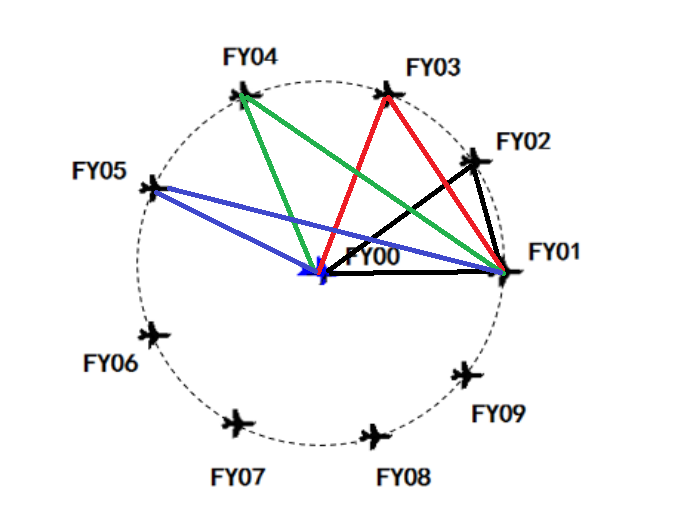
\includegraphics[width=0.6\textwidth]{pic1.png}
    \caption{发信机的位置情况} 
\end{figure}

由于太多的情况分类会导致模型的适用性有所下降,因此我们考虑不同的位置情况的通用描述量,即两架发信机与FY00形成的夹角。引入这个夹角作为模型的考虑变量,我们就将所有情况成功地在一个模型当中表达了出来。\\

2)接收机的位置关系

这里接收机的夹角取值范围是 $[0,\pi]$. 用 $\R^2$ 上的标准内积, 计算公式为
$$
    \angle BAC = \arccos (\frac{\langle A-B,A-C\rangle}{||A-B||_2||A-C||_2}),\quad A,B,C\in \R^2.
$$


\subsubsection{模型建立}

已知接收机与三架发射发信机形成的三个夹角, 接收机的位置可以被几乎唯一确定。
\begin{theorem}[定位基本定理]
    设 $O,A,B\in\R^2$ 互不相同, $\alpha,\beta,\gamma\in[0,\pi]$, 则满足 $\angle OCA = \alpha$, $\angle OCB = \beta$, $\angle BCA = \gamma$ 的点 $C$ 
    如果存在且不在过 $AOB$ 的圆上, 则 $C$ 能被唯一确定。
\end{theorem}
\begin{proof}
    满足 $\angle OCA = \alpha$ 的点 $C$ 的轨迹是圆弧或者直线. 考虑满足 $\angle OCA = \alpha$, $\angle OCB = \beta$ 的点 $C$. 
    利用 $OABC$ 不共圆, 这两个不重合圆弧
    或圆弧与直线或两条直线之间最多有两个交点. 若交点存在, 必有一个是 $O$, 而 $O$ 符合条件仅当 $\alpha=\beta=k\pi$. 
    此时 $O$ 是两直线的唯一交点. 否则, 符合条件的 $C$ 只可能为剩下一个交点或不存在. 
\end{proof}

若接收机机在理想位置附近,则接收机与三架发信机一定不共圆。接收机的位置就能被唯一确定。
通过引入发信机之间的夹角作为变量,我们考虑建立以下的基本数学模型:

\begin{figure}[H]
    \centering
    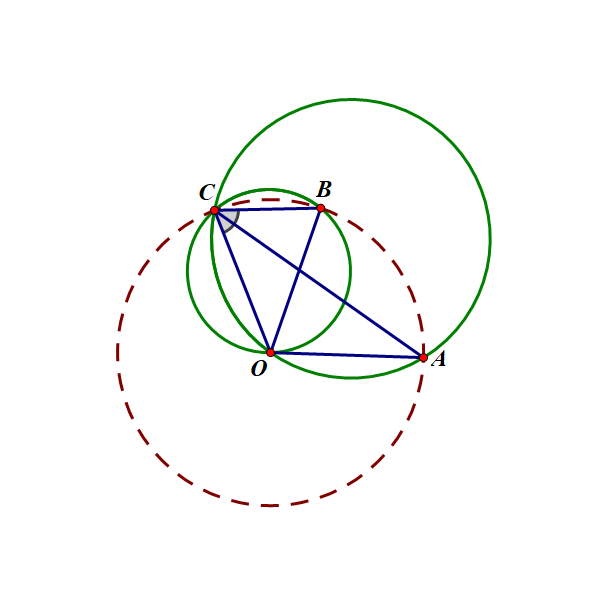
\includegraphics[width=0.5\textwidth]{sketch2}
    \caption{无人机定位系统的几何模型} 
\end{figure}

以 $O$ 为原点,$OA$ 为 $x$ 轴建立直角坐标平面,其中 $A$ 点的坐标为 $(r,0)$,$B$ 为另一架信号外机,设 $B$ 点的坐标为 $(rcos\theta,rsin\theta)$。同时,假设$\angle B C O = \beta$, $ \angle A C O = \alpha$。
由以上条件,得到 $AOC$ 的圆周方程:
$$
x ^ { 2 } + y ^ { 2 } - r x + \frac { r } { \tan \alpha } y = 0.
$$
同样,得到 $BOC$ 的圆周方程:
$$
x ^ { 2 } + y ^ { 2 } + ( - r \cos \theta - \frac { r \sin \theta } { \tan \beta } ) x + ( \frac { r \cos \theta } { \tan \beta } - r \sin \theta ) y = 0.
$$
利用两个圆弧的交点,我们得到 $C$ 点的坐标公式:
$$
x _ { c } = \frac { r A ^ { 2 } - r A / \tan \alpha } { A ^ { 2 } + 1 }, 
\quad y _ { c } = \frac { r A - r / \tan \alpha } { A ^ { 2 } + 1 }.
$$
其中:
$$
A = \frac { \frac { \cos \theta } { \tan \beta } - \sin \theta - \frac { 1 } { \tan \alpha } } { \cos \theta + \frac { \sin \theta } { \tan \beta } - 1 }.
$$

\subsubsection{模型求解}

通过基本的数学模型,我们设计算法对不同情况的点进行求解。考虑到接收机所处的位置不同,无法确定输入的角度的正负号,我们遍历一遍四种正负号的二元角度组,得到四个坐标定位。利用内积计算得到这四个坐标分别对应的三个夹角,与输入值比较,我们得以最终确定正确的坐标定位。于是,我们得到算法如下:

\begin{algorithm}[H]
\caption{\small 无人机定位算法}
\textbf{Input:} 接收的三个角度 $\alpha,\beta,\gamma$,两架信息外机的编号m,n,可接受误差限 $\delta$.\\
\textbf{Initialize:} $\theta=|m-n|\frac{2\pi}{9}$,$a^{(i)} = [\alpha,\alpha,-\alpha,-\alpha],b ^{(i)}= [\beta,-\beta,\beta,-\beta],O=(0,0),A=(1,0),B=(cos\theta,sin\theta),i=1$.\\
\textbf{Output:} 接收机的坐标 $(x,y)$ (单位为百米). \\
\textbf{Step1} 计算 $$N = \frac { \frac { \cos \theta } { \tan b^{(i)} } - \sin \theta - \frac { 1 } { \tan a^{(i)} } } { \cos \theta + \frac { \sin \theta } { \tan b^{(i)} } - 1 }.$$
\textbf{Step2} 计算 $$x= \frac { r N ^ { 2 } - r N / \tan a^{(i)} } { N ^ { 2 } + 1 } \quad y = \frac { r N - r / \tan ^{a(i)} } { N ^ { 2 } + 1 }\quad temp=(x,y).$$
\textbf{Step3} 计算 $$\alpha _ { t e m p } = \arccos ( \frac { ( temp  - A ) \cdot ( O - A ) } { | \operatorname temp - A | | O - A | } )$$ $$\beta _{ temp} = \arccos ( \frac { ( temp - B ) ( O - B ) } { | temp - B | | O - B | } )$$ $$\gamma_ { temp } = \arccos ( \frac { ( temp - A ) ( B - A ) } { |  temp - A | | B - A | } ).$$
\textbf{Step4} 如果存在 $|\alpha-\alpha_{temp}|\quad|\beta-\beta_{temp}|\quad|\gamma-\gamma_{temp}|$ 大于误差限 $\delta$, 则 $i=i+1$, 转至Step2, 直到满足误差限。
\end{algorithm}

\subsection{第二问:未知编号的无人机定位}
\subsubsection{小误差模型的建立与求解}
由于在不发生意外情况时,无人机相较于理想位置的偏差不会太大,因此我们首先考虑无人机的位置偏差足够小的情况。当在这个条件下,我们选择利用无人机的理想位置来确定无人机的编号。我们首先考虑三架无人机作为发信机的情况。通过理想位置的数据,我们计算出所有的角度信息三元组以及他们对应的发信机和接收机编号作为我们的信息库。

通过观察计算得到的三元组,我们发现,每个三元组都对应了至少两种发信机和接收机的编号情况,即两种不同的编号情况对应的接收信息完全相同,我们无法通过任何方式对它们进行区分。通过进一步计算四架及以上的发信机信息库,我们发现随着发信机数量的增加,同一个输入信息对应的编号情况也随之增加,无论选择几架发信机都无法对接收机进行有效定位。

为了解决这个问题,我们引入其他已知条件来增强我们的信息库:

1.接收机能够获取自己的编号信息。

2.接收机能够得知FY00和FY01对应形成的角度信息。

通过以上两个条件的限定,我们重新计算三架发信机形成的三元组$\{x^{i}\}$,并将FY00和FY01对应的角度信息放在三元组的第一位。获取输入信息$y$后,第一步,我们对比信息库当中的三元组和输入的角度信息三元组的第一位,即选择所有的$x^{(i)}$,满足:$$x ^ { ( i ) } = \operatorname { argmin } | x ^ { ( i ) }_1 - y_1 |$$

第二步,由于三个角度信息中,只有两个是独立的有效信息,因此我们删去所有三元组中最大的角度,防止冗余信息对模型的准确性产生未知的影响,最终生成信息库和输入信息对应的二元组。

第三步,我们通过计算范数来确定信息库当中和输入信息最接近的二元组,并结合接收机的编号,确定定位机的编号信息。由于范数的接近并不能够和距离的接近完全对等,因此我们考虑使用三种范数,即L1范数,L2范数和无穷范数,通过对比他们的正确率选择出合适的范数。

第四步,利用第一问的无人机定位算法,得到接收机的有效定位。

最终,我们得到完成的小误差定位算法如下:
\begin{algorithm}[H]
\caption{\small 小误差定位算法}
\textbf{Input:} 信息库$\{x^{(i)}\}$和对应的编号信息$\{m^{(i)}\}$,角度信息y,接收机编号n\\
\textbf{Output:} 接收机的有效定位\\
\textbf{Step1} 对所有$\{x^{i}\}$,筛选$x^{(i)}$满足$$x ^ { ( i ) } = \operatorname { argmin } | x ^ { ( i ) }_1 - y_1 |$$\\
\textbf{Step2} 对所有$\{x^{i}\}$,删除$$x _ { k } ^ { ( i ) } = \max ( x _ { j } ^ { ( i ) } ) \quad ( j = 1,2,3 )$$\\
\textbf{Step3} 选择$x^{(i)}$满足$$x ^ { ( i ) } = \operatorname { argmin } \| x ^ { ( i ) } - y \| _  { p }\quad ( p = 1,2 , \infty )$$\\
\textbf{Step4} 查找$x^{(i)}$对应的编号信息,同时满足$$m^{(i)}_2=n$$\\
\textbf{Step5} 调用无人机定位模型(Algorithm1)计算接收机位置\\
\end{algorithm}

利用小误差定位算法,我们模拟了偏差率最大值为20\%的情况。模拟流程如下:由于对称性,我们通过python并对发送机为2,3,4,5的情形进行模拟。我们对除发送机外所有的点调整20\%误差,以4\%误差率为间隔点遍历所有可能的分布,给他发信机的三个角度信息,接收机不知道第三台发射机的编号,但他知道FY00-FY01组成的夹角,如果他能够通过这三个角的信息正确推断出FY00,FY01外的第三台发送机的编号,那么我们认为它能够有效定位,将该位置标记为红点。如果他推断错误,则标记为蓝点。就得出了下面三张三种范数计算下的偏差推断分布图:

\begin{figure}[H]
    \centering
    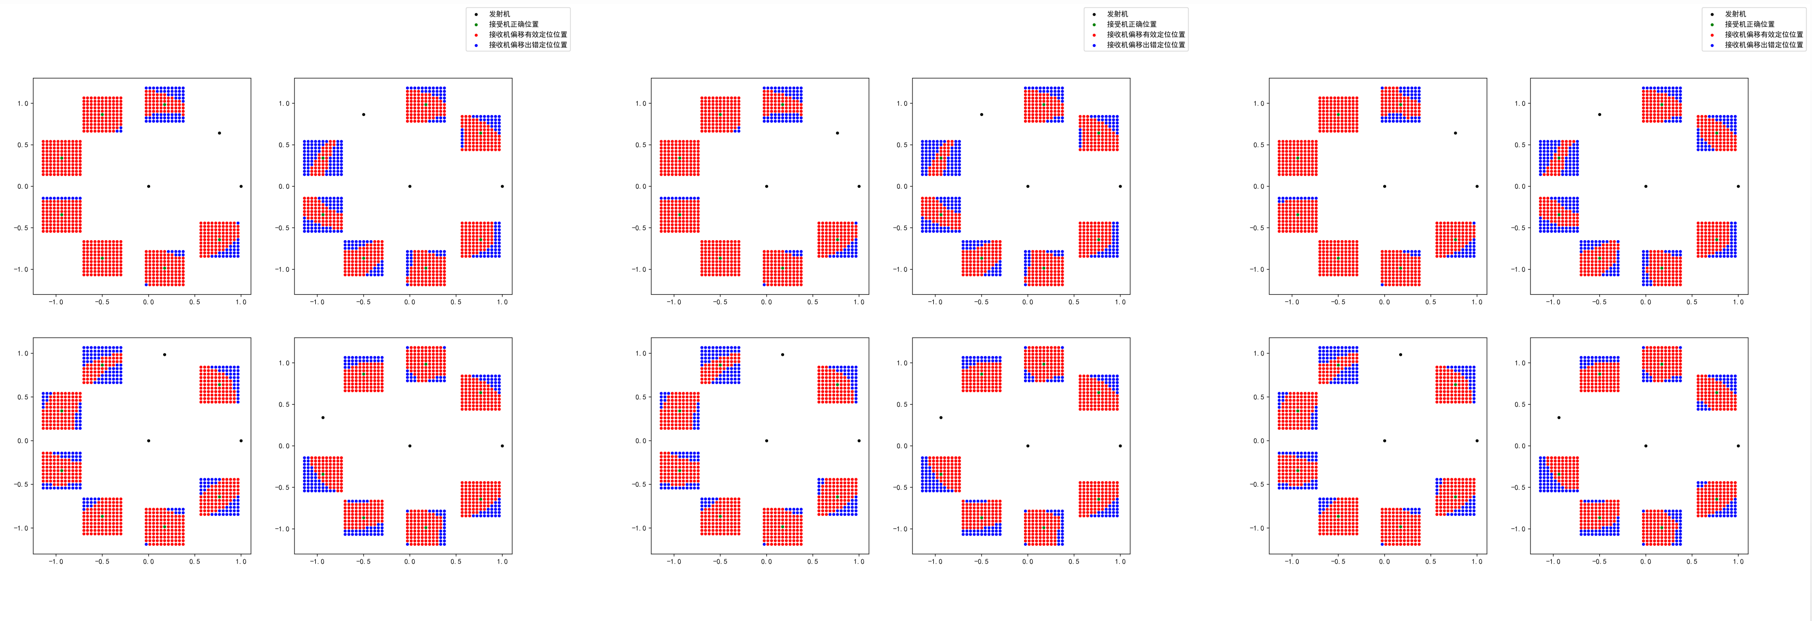
\includegraphics[width=1\textwidth]{two}
    \caption{基于不同范数的无人机定位} 
\end{figure}

通过观察结果我们发现,L1范数和L2范数的结果要好于无穷范数,并且三种范数都能在误差小于6\%的情况下对接收机做出完全准确的定位,随着误差限的增加,仍然能够保持比较高的正确识别率。因此,在误差足够小的情况下,三架发信机就能产生有效定位。


\subsubsection{大误差模型的建立与求解}
当无人机没有误差限制的时候,我们完全无法确定发信机的编号,由于没有角度的限制,相同的输入信息对于每一种发信机组合都能够得到一个定位。并且由于角度信息的所属关系的不确定,随着发信机的数量增加,系统的混沌程度也随之上升,因此在无误差限制的情况下想要完全确定无人机的定位是不可能的。在这种情况下,我们希望尽可能增加正确判断无人机位置的范围基于无人机偏离理想位置过大的可能性较低的事实,我们引入一个新的条件,即无人机的可能位置以无人机的理想位置为中心,呈二维正态分布的随机状态。

在这样的条件下,我们认为无人机的实际位置接近自身的理想位置越近,概率越大,因此我们通过角度信息和所有包含FY00和FY01在内的三架发信机组合,计算出接收机实际位置可能的点位,通过计算这些点位和接收机理想位置的欧几里得范数,找到最接近理想位置的点位,并以这个点位作为无人机的有效定位。

以这个想法为基础,我们对其进行规范化和量化,得到大误差定位算法如下:
\begin{algorithm}[H]
\caption{\small 大误差定位算法}
\textbf{Input:} 接收到的角度信息y,接收机的编号k,接收机理想位置$q_0$\\
\textbf{Output:} 无人机的位置q\\
\textbf{Step1} 调用无人机定位算法(Algorithm1),对所有$j\in\{2,3,4,5,6,7,8,9\}$且$j\neq k$,以FY00,FY01,FY0j作为发信机计算无人机位置序列$\{q^{(j)}\}$\\
\textbf{Step2} 选择$q^{(j)}$满足$$q ^ { ( j ) } = argmin \| q_0 - q ^ { ( j ) } \| _ { 2 }$$ \\
\textbf{Step3} 决定$q^{(j)}$作为无人机的实际位置$$q= q ^ { ( j ) }$$
\end{algorithm}

利用大误差定位算法,我们对无人机的定位情况进行模拟模拟流程如下:

对于二维正态分布,我们假定x,y不相关并且x,y的标准差相等。
由于对称性,我们通过python对发送机为2,3,4,5的情形进行模拟。选定发送机后,我们随机选择一台接收机的编号,在二维正态分布上随机取点,并向它发送三个角度信息。我们接着将接收到的角度信息与其他不同的发信机组合联立,得到其余的错误定位点。

如果是最开始定位点与理想位置的的距离是最小的,那么我们认为这是一次可靠的定位,画作红点,反之则认为不可靠,画作蓝点。首先假设标准差为0.1,对于每种情形我们测试了100次,得到的分布图如下所示:

\begin{figure}[H]
    \centering
    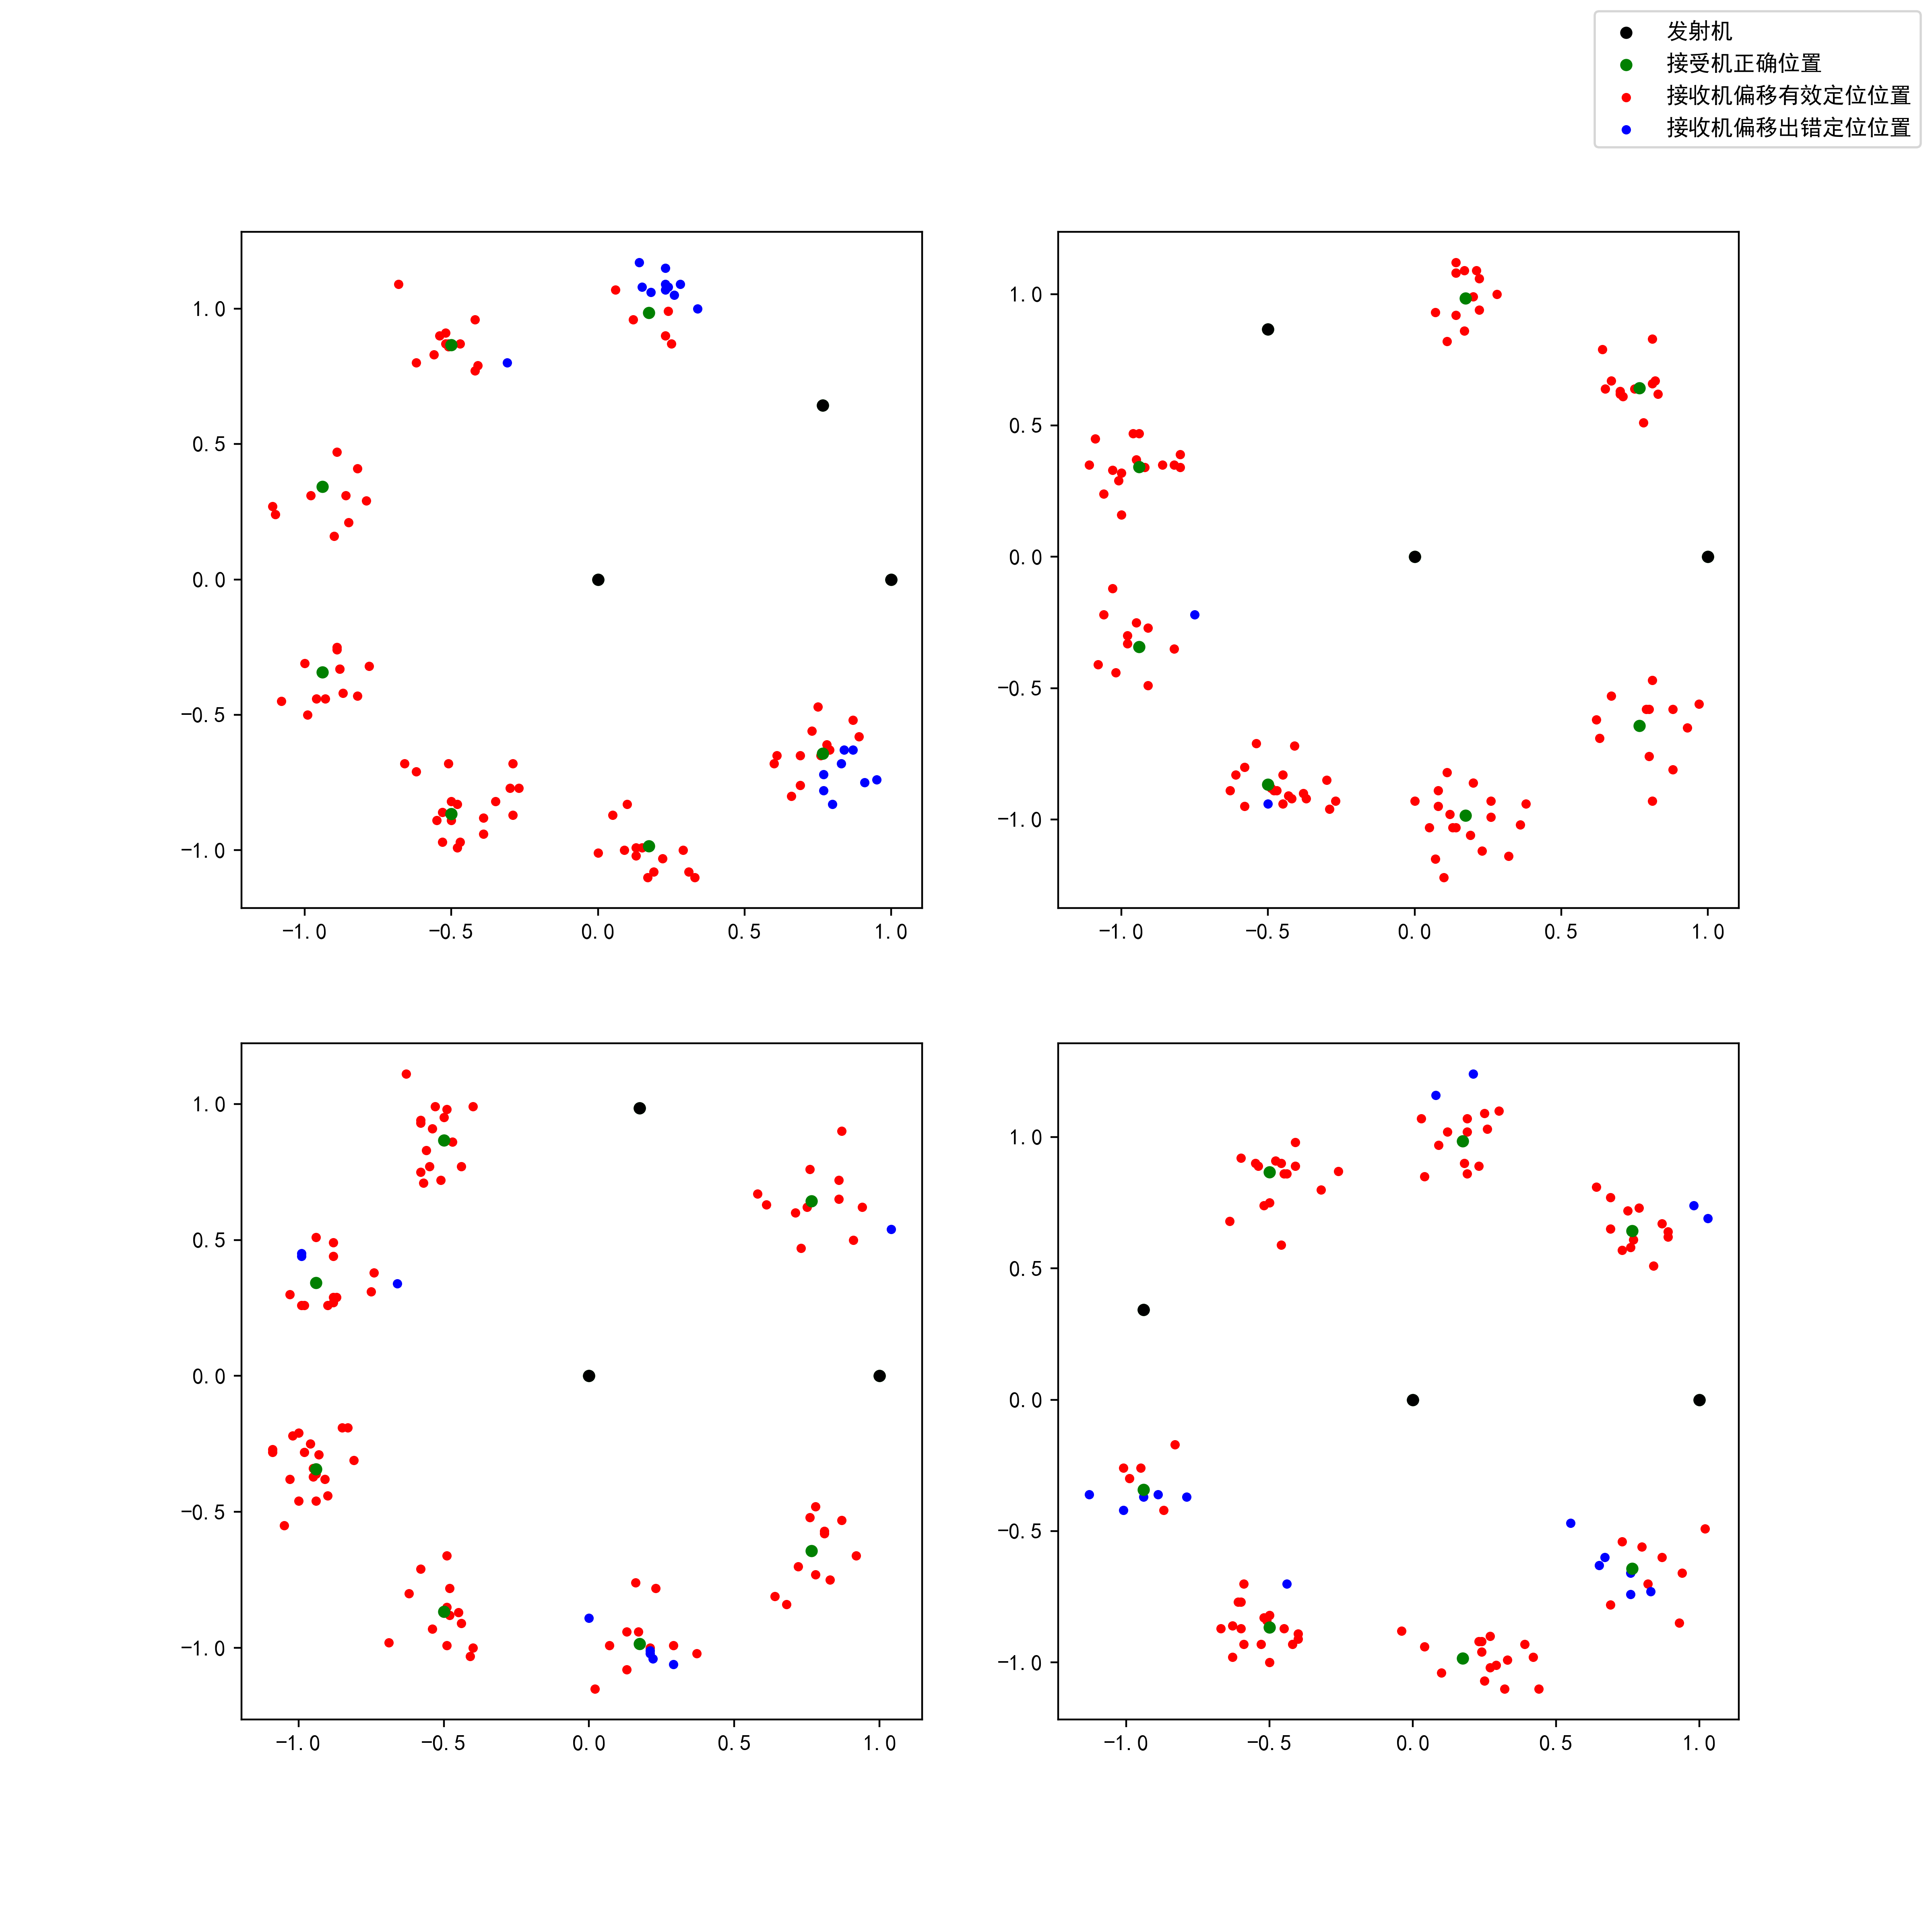
\includegraphics[width=0.7\textwidth]{two0}
    \caption{大误差无人机定位} 
\end{figure}

可以看到,我们的数据图在大部分情况下都呈现红色,正确率较高,所以在标准差0.1的正态分布下,该算法是较为可靠的。

\subsection{第三问模型的建立与求解}
    注意到理想情况下FY01,FY04,FY07构成一个等边三角形,FY00是它的中心。第一步我们将固定FY00和FY01,
    通过反复调整FY04和FY07,使得FY01,FY04,FY07构成以FY00为中心的等边三角形。下面的定理保证了这样
    调整进行得很快。
\begin{theorem}[等边三角形定理]
\label{dbsjx} 
    设 $O=(0,0)$, $C=(1,0)$,   
    $A^{(0)}=(1+\Delta,-\frac{2\pi}3-\delta)\in \R^{\geq 0}\times S^1$. 用如下递归的方式构造点列
    $\{B^{(i)}\}_{i\geq 1}$, $\{A^{(i)}\}_{i\geq 1}$: 
    $B^{(i)}=(r_B^{(i)},\theta_B^{(i)})$, $\theta_{B}^{(i)}\in (\frac \pi 2,\pi)$ 是
    第二象限中满足 $\angle CB^{(i)}O=\angle OB^{(i)}A^{(i-1)}=\frac\pi6$ 的点, 
    $A^{(i)}=(r_A^{(i)},-\theta_A^{(i)})$, $\theta_{A}^{(i)}\in (\frac \pi 2,\pi)$ 是
    第三象限中满足 $\angle CA^{(i)}O=\angle OA^{(i)}B^{(i)}=\frac\pi6$ 的点(接下来构造 $B^{(i+1)}$, $A^{(i+1)})$. 
    则 
    \begin{equation}
    \begin{aligned}
        r_A^{(i)}=1+o((|\Delta|+|\delta|)^{(i)}),\quad r_B^{(i)}=1+o((|\Delta|+|\delta|)^{(i-1)}),
        \\
        \theta_A^{(i)}=\frac{2\pi}{3}+o((|\Delta|+|\delta|)^{(i)}),\quad \theta_B^{(i)}=\frac{2\pi}{3}+o((|\Delta|+|\delta|)^{(i-1)}).
    \end{aligned}
    \label{1}
    \end{equation}
    利用有限维 Banach 空间的范数等价性, 有序列 $A^{(i)}$, $B^{(i)}$ 分别依2-范数超线性收敛到
    (converge superlinearly\cite{dennis1974characterization} under Euclidean norm to) $(1,\frac{-2\pi}3)$, $(1,\frac{2\pi}3)$.
\end{theorem} 

\begin{figure}[H]
    \centering
    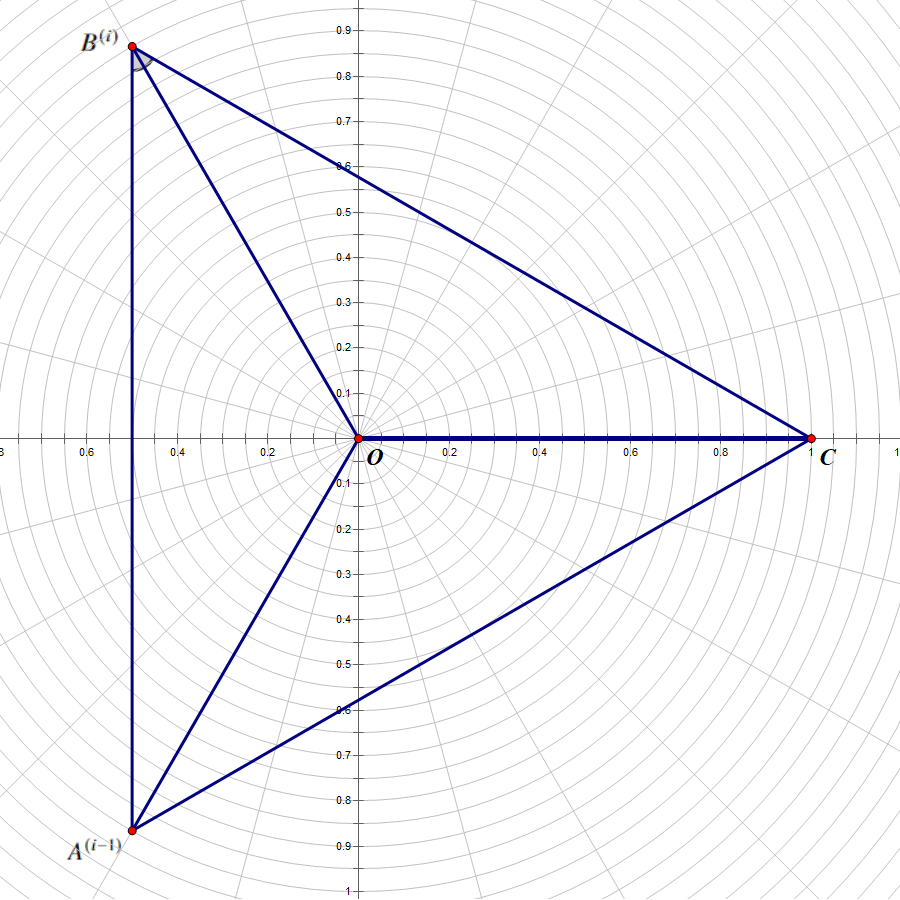
\includegraphics[width=0.5\textwidth]{sketch1}
    \caption{从 $A^{(i-1)}$ 构造 $B^{(i)}$ 的过程} 
\end{figure}

\begin{proof}
    不妨设 $r_A^{(i-1)}=1+\Delta_A^{(i-1)}$, $\theta_A^{(i-1)}=\frac{2\pi}{3}+\delta_A^{(i-1)}$. 根据几何关系,有 
    $$
    r_A^{i-1}\sin(\theta_B^{(i)}+\theta_A^{(i-1)}-\frac{7\pi}{6})=\sin(\frac{5\pi}{6}-\theta_{B}^{(i)})=\frac12 r_B^{(i)}.
    $$
    做 Taylor 展开,忽略一阶小就有
    $$
        \theta_{B}^{(i)}= \frac{2\pi}3-\frac{1}{2} \delta_A^{(i-1)}-\frac{\sqrt 3}6 \Delta_A^{(i-1)}+o(|\Delta_A^{(i-1)}|+|\delta_A^{(i-1)}|)
        ,\quad r_{B}^{(i)} = 1 +\frac{\sqrt3}{2} \delta_A^{(i-1)}+\frac12 \Delta_A^{(i-1)}+o((|\Delta_A^{(i-1)}|+|\delta_A^{(i-1)}|).
    $$
    利用旋转对称性,可得
    \begin{equation}
    \begin{aligned}
        \theta_{A}^{(i)}= \frac{2\pi}3-\frac{1}{2} (-\frac{1}{2} \delta_A^{(i-1)}-\frac{\sqrt 3}6 \Delta_A^{(i-1)})
        -\frac{\sqrt 3}6 (\frac{\sqrt3}{2} \delta_A^{(i-1)}+\frac12 \Delta_A^{(i-1)}) +o(|\Delta_A^{(i-1)}|+|\delta_A^{(i-1)}|)
        \\=o(|\Delta_A^{(i-1)}|+|\delta_A^{(i-1)}|).&
    \end{aligned}
    \label{2}
    \end{equation}
    同理 $r_{A}^{(i)}=o(|\Delta_A^{(i-1)}|+|\delta_A^{(i-1)}|).$ 利用数学归纳法可得结果. 
\end{proof}

    利用调整两个夹角为 $\frac\pi6$ 的方式,上面的定理保证了 FY04 和 FY07 能被快速地调整到理想位置。
    接下来我们假定 FY04 和 FY07 的位置正确,通过第一小问的方法即可定位所有其他飞机并调整他们到理想位置。

\begin{algorithm}[H]
    \caption{\small 无人机位置调整算法}
    \textbf{Input:} 预计无人机位置与理想位置的径向绝对误差 $\Delta$, 角向绝对误差 $\delta$, 可接受误差限 $\delta_0$.\\
    \textbf{Initialize:}. $r=1$.\\
    \textbf{Output:}. 无人机的正确位置.\\
    \textbf{Step1} 调整 FY04 的位置, 使得 FY04接收到的角度信息为 $\frac{\pi}{6}$,$\frac{\pi}{6}$,$\frac{\pi}{3}$.\\
    \textbf{Step2} 调整 FY07 的位置, 使得 FY07接收到的角度信息为 $\frac{\pi}{6}$,$\frac{\pi}{6}$,$\frac{\pi}{3}$.\\
    \textbf{Step3} 如果$(|\Delta|+|\delta|)^r\geq\delta_0$,回到 Step1,$r=r+1$,直到满足可接受误差限.\\
    \textbf{Step4} 对 $j\in\{2,3,5,6,8,9\}$, 计算 FY0j 在理想位置相对于 FY07, FY00, FY01 的夹角,并调整 FY0j 使得它与 FY07, FY00, FY01 的夹角与理想情况一致.\\
\end{algorithm}

利用无人机位置调整算法,我们将题目中给出的表1数据代入模型,得到如下图所示的调整过程:

\begin{figure}[H]
    \centering
    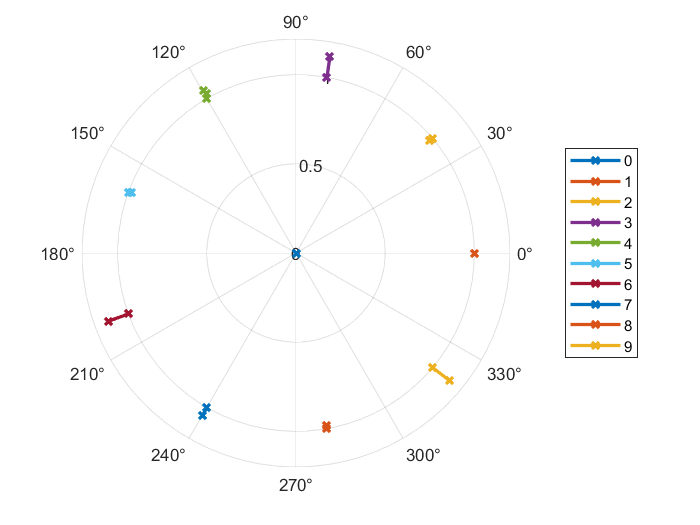
\includegraphics[width=0.6\textwidth]{three}
    \caption{表1无人机编队调整过程} 
\end{figure}

到所有无人机归位,我们一共只进行四次信号发射,大大减少了无人机收到外界干扰的可能性,因此我们认为模型比较优秀。

\subsection{问题二:无人机编队的调整}

\subsubsection{模型建立}
第三问的算法提供了一种调整位置的优秀方案,只要无人机队形中能找到一个接近等边三角形和它的中心的四架飞机,就可以很快地
将他们调整到合适的位置,以便其他飞机参照。因此对于飞机队形的调整问题,我们仍延续上一问的思路。

首先固定三架发信机 $A$, $O$, $B$, 接收机 $C$ 按照 $COB$ 
都处于理想位置时计算得到的理想角度进行调整。由于我们仅考虑相对角度和距离,不妨设 $O$, $C$ 处于理想位置。
考虑到 $B$ 可能有偏差, 此时 $A$ 与理想位置之间也会有些许偏差。
然后再用同样的方法调整 $A$ 的位置,此时 $BOC$ 作为发信机。如此重复下去相互调整 $B$, $A$ 位置。下面的定理保证了
只要 $B$, $C$ 的初始位置接近理想位置,且四架飞机之间的位置关系满足一定条件,这样的调整方案是收敛的。此外,
定理还给出了快速收敛时四架飞机位置需要满足的条件。定理可以自然地推出等边三角形定理。
这个定理有一定的技术性,在此省略了部分计算过程,但是其证明思想与等边三角形定理一致。 
\begin{theorem}[三角形内点调整法收敛判据]
    \label{remarkable}
    设 $O=(0,0)$, $C=(1,0)$. 取 $A_0=(r_A, -\theta_A)$, $B_0 = (r_B,\theta_B)$ 为目标位置, 点 $O$ 位于
    三角形 $A_0B_0C$ 的内部.
    固定 $\angle OCB_0=\alpha_1$, $\angle OCA_0=\beta_1$, $\angle OB_0A_0=\alpha_2$, $\angle OB_0C=\beta_2$,
    $\angle OA_0C=\alpha_3$, $\angle OA_0B_0=\beta_3$,  
    用如下递归的方式构造点列 $\{B^{(i)}\}_{i\geq 1}$, $\{A^{(i)}\}_{i\geq 1}$: 先找到
    $B^{(i)}=(r_B^{(i)},\theta_B^{(i)})$ 满足 $\angle A^{(i-1)}B^{(i)}O=\alpha_2, \angle CB^{(i)}O=\beta_2$, 再找到
    $A^{(i)}=(r_A^{(i)},-\theta_A^{(i)})$, 满足 $\angle CA^{(i)}O=\alpha_3, \angle OA^{(i)}B^{(i)}=\beta_3$. 如此重复下去.
    设 
    $$
        Z = \frac{(\cot \beta_3-\cot\beta_1)(\cot \alpha_2-\cot \alpha_1)}
        {(\cot \alpha_1+\cot \beta_3)(\cot \alpha_2+\cot \beta_1)}.
    $$
    若 $|Z|< 1$ 则点列 $A^{(i)}$, $B^{(i)}$ 线性收敛(linearly convergent)到 $A_0$, $B_0$. 
    该收敛是超线性 (superlinear) 的当且仅当 $\alpha_2=\alpha_1$ 或 $\beta_3=\beta_1$. 
\end{theorem}
\begin{figure}[H]
    \centering
    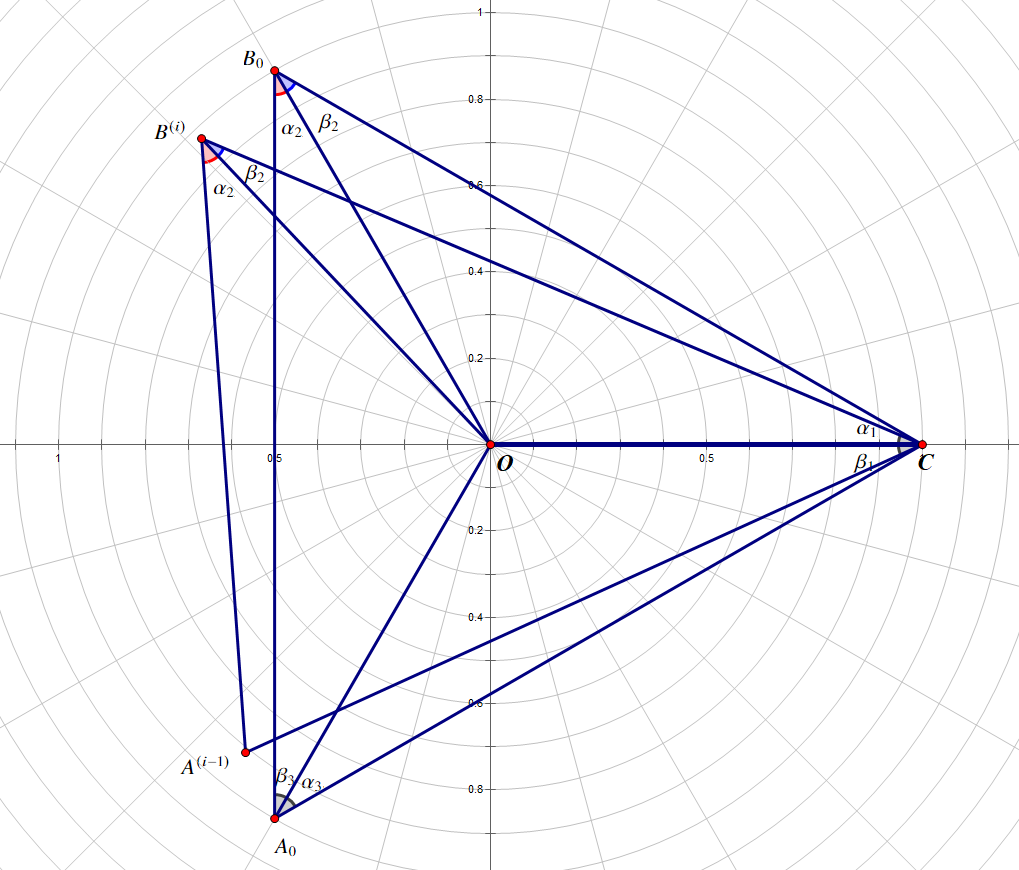
\includegraphics[width=0.6\textwidth]{sketch4}
    \caption{从 $A^{(i-1)}$ 构造 $B^{(i)}$ 的过程} 
\end{figure}
\begin{proof}
    这个定理是等边三角形定理的推广. 根据几何关系, 有
    $$
        \frac{1}{\sin\beta_2}=\frac{r_B^{(i)}}{\sin(\alpha_1+\theta_B-\theta_B^{(i)})},\quad
        \frac{r_A^{(i-1)}}{\sin\alpha_2} = \frac{r_B^{(i)}}{\sin(\beta_3-\theta_B+\theta_B^{(i)}-\theta_A+\theta_A^{(i-1)})}.
    $$
    做 Taylor 展开, 忽略高阶小, 有
    $$
        \theta_B^{(i)}-\theta_B = \frac{-\cot \alpha_2}{\cot\beta_3+\cot\alpha_1}(\theta_A^{(i-1)}-\theta_A)+
        \frac{-1}{\cot\beta_3+\cot\alpha_1}(r_A^{(i-1)}-r_A)+o(|\theta_A^{(i-1)}-\theta_A|+|r_A^{(i-1)}-r_A|),
    $$
    且 
    $$
        r_B^{(i)}-r_B= -\cot\alpha_1(\theta_B^{(i)}-\theta_B)+ o(|\theta_A^{(i-1)}-\theta_A|+|r_A^{(i-1)}-r_A|).
    $$
    设 
    $$
    X=\frac{\cot \beta_3(\cot \alpha_2-\cot \alpha_1)}
    {(\cot \alpha_1+\cot \beta_3)(\cot \alpha_2+\cot \beta_1)},\quad
    Y=\frac{(\cot \alpha_2-\cot \alpha_1)}
    {(\cot \alpha_1+\cot \beta_3)(\cot \alpha_2+\cot \beta_1)}.
    $$
    代入上一步的误差项迭代, 就有
    $$
    \theta_A^{(i)}-\theta_A = X(\theta_A^{(i-1)}-\theta_A) + Y(r_A^{(i-1)}-r_A) + o(|\theta_A^{(i-1)}-\theta_A|+|r_A^{(i-1)}-r_A|).
    $$
    和
    $$
    r_A^{(i)}-r_A= -\cot\beta_1X(\theta_A^{(i-1)}-\theta_A)-\cot\beta_1Y(r_A^{(i-1)}-r_A)+ o(|\theta_A^{(i-1)}-\theta_A|+|r_A^{(i-1)}-r_A|).
    $$
    写成矩阵形式, 就有
    $$
        \begin{pmatrix}
            \theta_A^{(i)}-\theta_A\\
            r_A^{(i)}-r_A
        \end{pmatrix}
        =
        M
        \begin{pmatrix}
            \theta_A^{(i-1)}-\theta_A\\
            r_A^{(i-1)}-r_A
        \end{pmatrix},
        \quad
        M=
        \begin{pmatrix}
            X&Y\\
            -\cot\alpha_2 X& -\cot\alpha_2 Y\\
        \end{pmatrix}
        +o(|\theta_A^{(i-1)}-\theta_A|+|r_A^{(i-1)}-r_A|).
    $$
    因为 $\sigma_M=\{0, X-\cot\beta_1 Y\}$ ( $\sigma_M$ 表示矩阵 $M$ 的谱), 令 $Z=X-\cot\beta_1Y$. 
    若 $|Z|<1$, 则点列 $A^{(i)}$, $B^{(i)}$ 线性收敛(linearly convergent)到 $A_0$, $B_0$. 
    该收敛是超线性 (superlinear) 的当且仅当 $\alpha_2=\alpha_1$ 或 $\beta_3=\beta_1$. 
\end{proof}

    对于给定的飞机队形,我们首先找到满足定理条件的四架飞机,用定理给出的方式调整位置。进行足够多次迭代后,再利用调整好的飞机确定其他飞机的位置。
    我们给出一些满足 $\alpha_1=\alpha_2$ 或 $\beta_1=\beta_3$ 的图形。可以发现,在一般的规则队形中,这样的图形是常见的,例如题目中给出的锥形编队。
\begin{figure}[H]
    \centering
    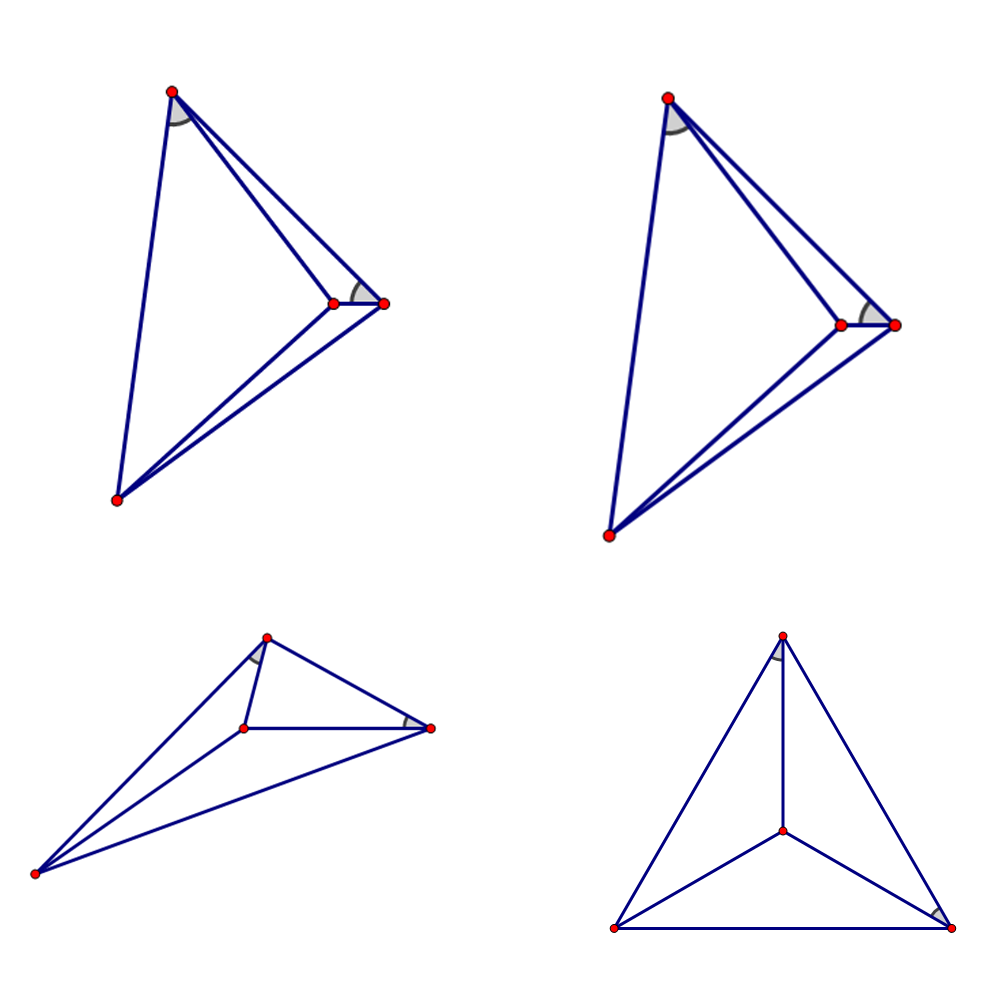
\includegraphics[width=0.5\textwidth]{four1}
    \caption{超线性收敛的例子} 
\end{figure}

    如果找不到这样的图形,我们可以找到 $|Z|$ 最小即收敛速度最快的调整方法。

\subsubsection{模型求解}
利用我们推广后的基本模型,我们只需要在编队当中搜索包含内机的三角形,再计算得到他们之中矩阵特征值最小的那个。以这个三角形的四架组成无人机作为定位机,重复无人机算法,即可完成对所有无人机的定位。

由于三架外机两两都可以作为一对调整组合,因此我们首先对一个含内机的三角形所包含的三个矩阵进行对照,选择出其中特征值最小的一个,如果它的特征值小于1,那么就将它放入队列。

另一方面,由于一些极少数的特殊情况,为了防止出现矩阵特征值小于一却无法收敛的情况出现,我们将存储的三角形队列按对应特征值的大小从小到大排列,依次进行收敛性模拟,直到有满足收敛条件的三角形出现,或是队列中的所有三角形都不满足条件。于是,我们得到算法流程图如下:

\begin{figure}[H]
    \centering
    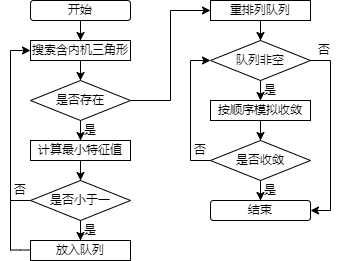
\includegraphics[width=0.5\textwidth]{four2}
    \caption{编队调整算法流程} 
\end{figure}

在搜索到可收敛的含内机三角形后,我们就可以调用无人机位置调整算法(Algorithm4)来完成编队的调整。如果搜索不到可收敛的三角形,则编队无法快速调整。

问题二中给出的锥形例子中,FY01,FY05,FY07,FY10构成了等边三角形和重心,因此只需要按照第三问的方法进行调整就行。我们考虑顶角为九十度的锥形,利用算法进行搜索和调整,得到调整仿真图如下:

\begin{figure}[H]
    \centering
    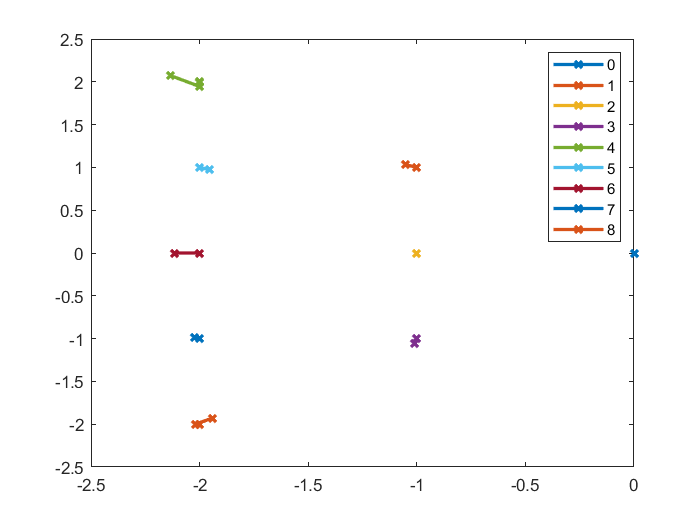
\includegraphics[width=0.6\textwidth]{four3}
    \caption{问题二模型结果} 
\end{figure}

由于九十度的锥形最小特征值不为零,为线性收敛,共调整了七次,高于第三问编队的超线性收敛,但仍然满足收敛条件。

%----------- 六、模型的分析与检验 ----------
\section{六、模型检验与灵敏度分析}
\subsection{第一问的模型检验}
我们设计相应的测试对我们的算法模型进行测试以验证算法的正确性。测试方案如下:

对于发送机不同夹角的4种情况进行测试模拟。选定R = 1。每次测验通过计算机随机选定一台编号的接收机,我们认为他的位置距离他的理想位置至多有ErrorRate的误差。通过坐标的计算,程序会给接收机提供三个发信机的三个角度信息来模拟真实场景,接收机得到该角度信息后,通过第一问得到的算法,算出自身的x轴坐标以及y轴坐标,与计算机选定的真实坐标进行比对,如果两者的差值小于误差$(10^{-5})$,我们认为这次定位正确的,红点是能够准确定位的点,而蓝点则表示定位失败。重复上述测验100次,计算出程序定位的错误率。\\
测试结果如下图显示(ErrorRate=20\%):
\begin{figure}[H]
    \centering
    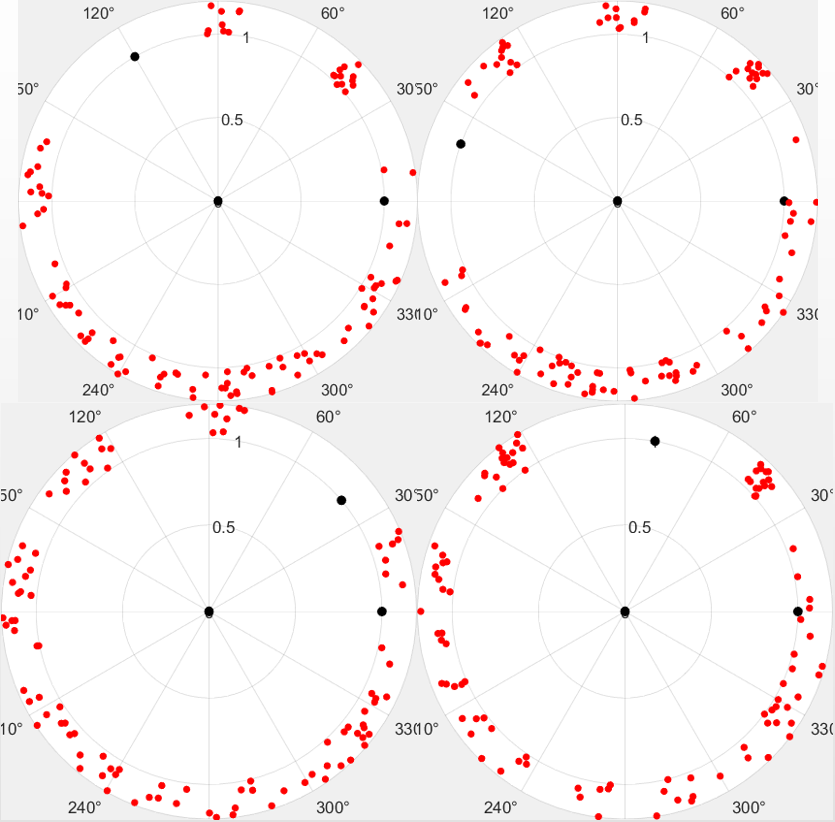
\includegraphics[width=0.6\textwidth]{check1}
    \caption{第一问模型检验} 
\end{figure}

上图为ErrorRate=20\%的测试图,红色的点是随机测试能够正确定位的点,黑色的是发射机,他的位置没有偏差。由于情况是对称的,因此4种情况便能模拟所有可能的情形。通过结果检验,我们的模型在20\%的误差限时能够完全定位无人机的位置。我们接着改变误差率ErrRate,当增大误差范围的时候,除开接收机与两台无人机形成三点一线的特殊情形,我们的模型都能够对无人机做出正确的定位,因此正确率几乎不受偏差限的影响。因此我们认为定位算法是有效且稳定的。\\

\subsection{第二问的模型检验}
\subsubsection{小误差定位的模型检验}
在小误差定位算法的模型求解结果下,我们进一步对模型进行灵敏度分析,进行不同范数下偏差率-算法正确率的计算,来判断哪个范数的效果最好,以及偏差率对算法正确率的影响。模拟流程如下,对发送机为2,3,4的情形进行模拟,每种情形测试每台接受机该误差率下的8个点进行定位,对所有情形正确总数除上测试总数来计算正确率,我们得到不同范数的偏差率-算法正确率如下:

\begin{figure}[H]
    \centering
    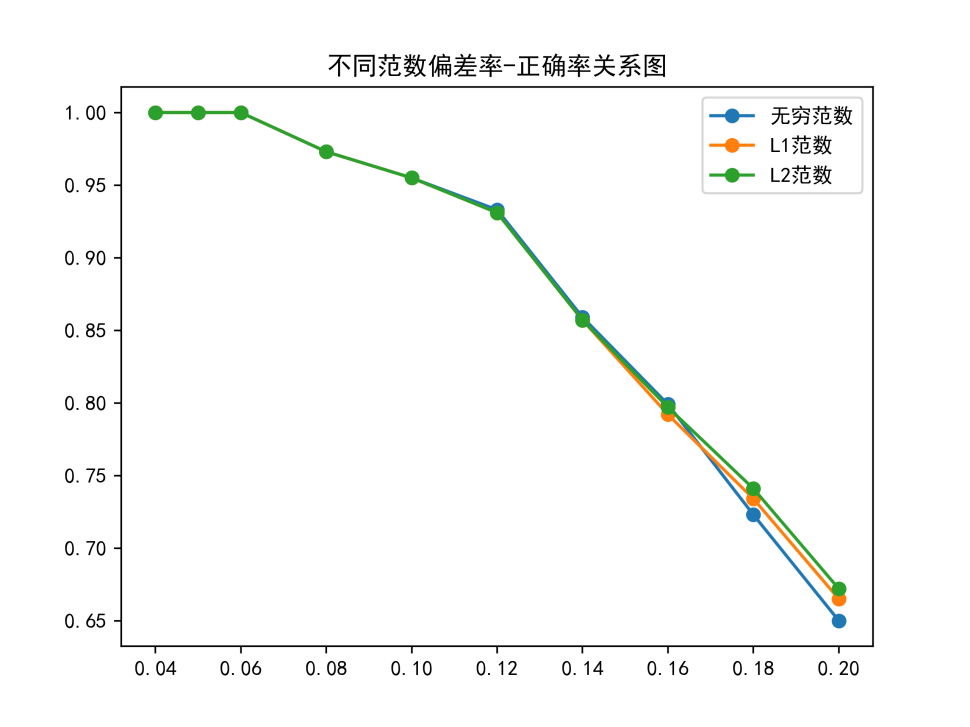
\includegraphics[width=0.7\textwidth]{check2}
    \caption{小误差灵敏度分析} 
\end{figure}

从图中可以发现,在偏差值较小时,正确率为100\%,算法是可靠的,当误差率上升时,算法定位的正确率下降。并且比较不同范数,随着偏误率增大,L2范数的正确率下降更为缓慢,更为稳定,L1范数次之,无穷范数的表现最差。在20\%偏误率时,正确率也最高,因此得出结论:L2范数的效果最好,基于L2范数的算法是最为合适的。同时,我们发现在13\%的误差率以下时,我们的模型正确率受偏差率影响不大,能够保持在接近95\%的正确率,因此我们认为我们的模型是有效且稳定的。
\subsubsection{大误差定位的模型检验}

大误差模型在正态分布标准差为0.1的情况下得到了较好的结果,因此我们希望更进一步,通过调整正态分布的标准差,即无人机有更大的可能严重偏离理想位置的情况下,考察我们标准差对我们模型结果的影响,对模型进行灵敏度分析。

\begin{figure}[H]
    \centering
    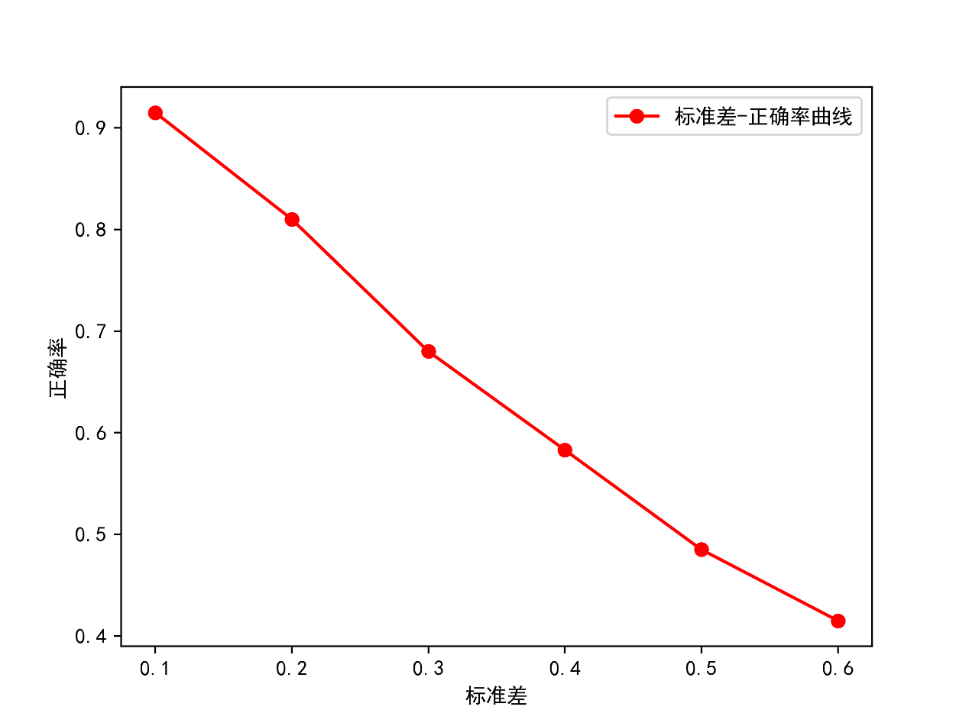
\includegraphics[width=0.7\textwidth]{check22}
    \caption{大误差灵敏度分析} 
\end{figure}

我们测试了0.1-0.6的6个标准差,得到的结果如上图所示。可以看到,我们的模型在标准差较小时有着较高的解释率。但是当标准差过大时,随着系统的混沌程度提高,模型的正确率就越低。因此我们可以得到结论:随着二维正态分布x和y标准差的增大,无人机离正确位置偏移较远的概率越大,就越可能导致算法的不可靠,算法的正确率越低。

\subsection{第三问的模型检验}
第三小问我们选择等边三角形的构造来实现编队的调整,并对表1的数据给出了具体的调整方案。为了测试模型的可靠性,我们选择来构造类似的圆形编队数据来验证该算法的正确性。由于情况对称,我们选择正确点为F00,F01,其他接收机偏差范围为10\%对算法进行验证。因为只要三架无人机的编号确定,其余所有飞机都可以根据这三架飞机来进行定位,所以算法的正确性只需要验证1,4,7三架飞机根据我们的调整方案能否组成等边三角形,我们认为只要在10次调整之内调整成功,则这次调整就是正确的。
测验数量为100次,可以得到结果为正确率100\%,而偏差率10\%的情况下调整次数约为4.8次,而下面是其中两张随机点的收敛图,数据同样在q3.m。因此我们得出结论,我们的模型有极强的普适性,在误差范围一定时都能够适用,并且收敛速度极快。

\begin{figure}[H]
    \centering
    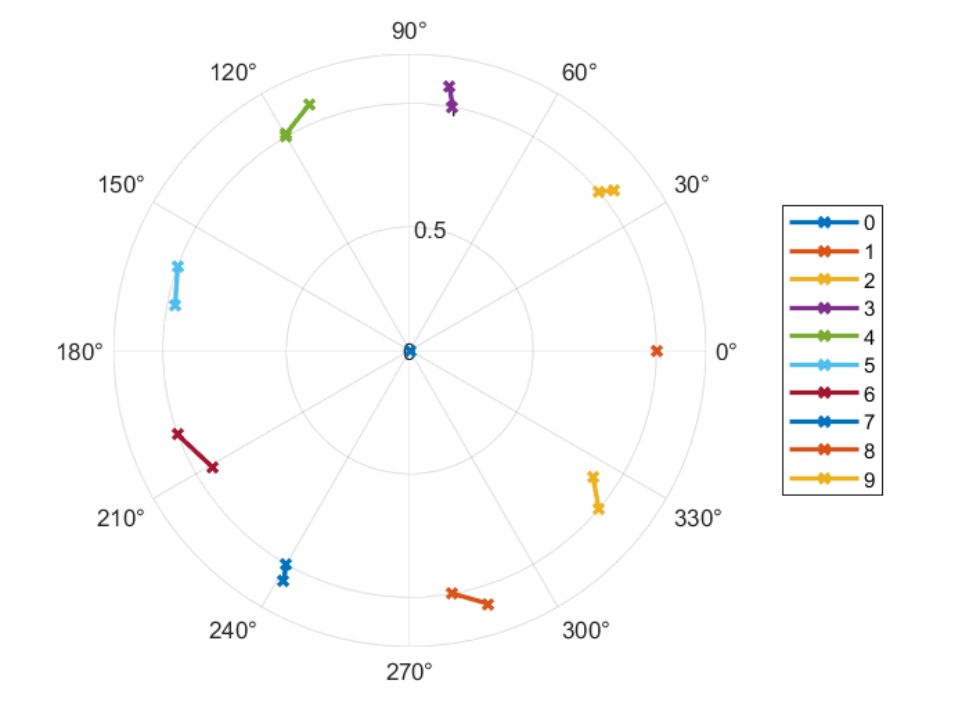
\includegraphics[width=0.7\textwidth]{check3}
    \caption{无人机调整模型验证} 
\end{figure}

\subsection{问题二的模型检验}

我们选择了一组特征值为零的系统和一组特征值较大的系统,对它们做调整仿真来验证我们的模型:

\begin{figure}[H]
    \centering
    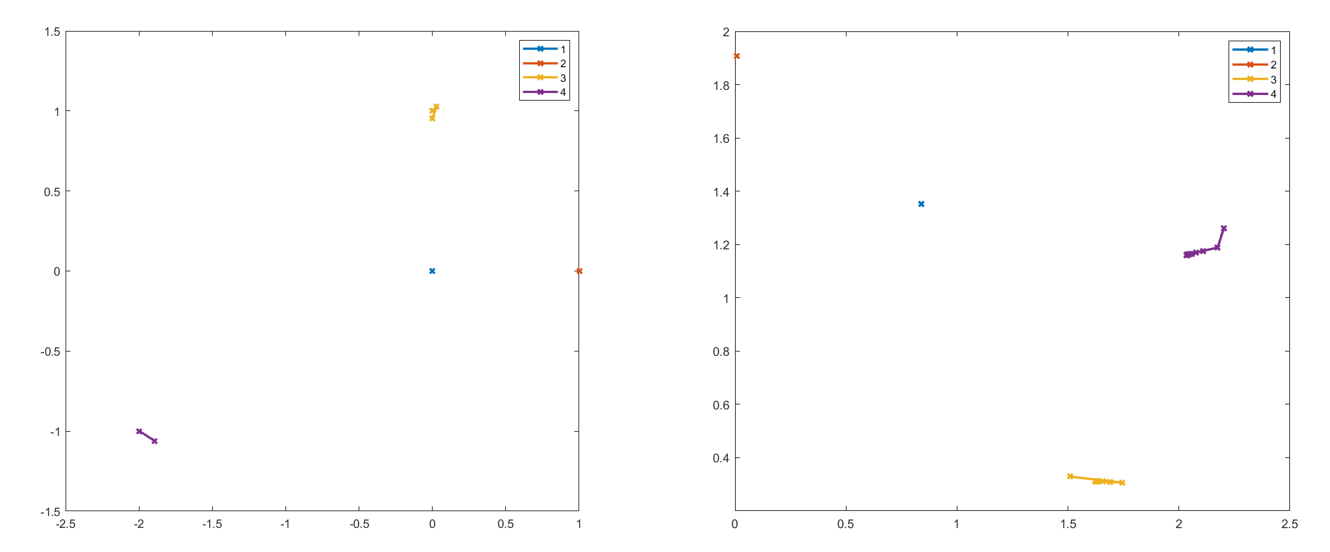
\includegraphics[width=0.9\textwidth]{check4}
    \caption{编队调整模型验证} 
\end{figure}

通过观察对比两个结果,我们可以发现,特征值较大的收敛次数多,但是仍然满足收敛条件,这验证了我们的模型。

\section{七、模型的评价、改进与推广}
\subsection{模型的优点}
1.无人机编队调整算法基于基本的几何模型,并且推广到了一般的含内机三角形,在无人机

\quad 编队问题中具有极强的普适性,能够直观的给出任意无人机编队的可调整性,为无人机编

\quad 队队形的选择提供了帮助。

2.定位和调整模型都在基本模型之上考虑了实际情况,给出了详细的算法,让模型具有更强

\quad 的可操作性和实现能力,能够更好地运用于实际的无人机编队飞行情况。
\subsection{模型的缺点}
1.在调整模型当中仅考虑到了无人机的目的地确定,而没有考虑到无人机的调整寻找路径能

\quad 力,需要无人机自行调整到正确的角度位置上,可能导致无人机调整花费的工作较多,浪费

\quad 编队行进的时间。

2.定位和调整模型在大误差下的解释率较低,当出现意外情况导致编队队形出现严重变化且

\quad 丢失编号信息时,无法对编队当中的无人机进行有效的定位和队形调整
\subsection{模型的改进}
一个方面,我们可以利用无人机的定位情况和理想位置建立无人机的最短寻路系统,在发信机位置不确定正确的情况下给出一个选择路线可能的最优方案,让无人机能够更加方便地寻找到自己的目标位置,缩短调整时间,提高无人机编队的效率。另一方面,可以建立不同情况下误差率与正确率的准确关系,为无人机的编队调整提供参考。
\subsection{模型的推广}
根据我们的三角形调整收敛定理,我们可以将这个收敛性向更多的由四个点组成简单几何图形推广。例如现在的定理要求我们必须要有一个内点,我们可以尝试将定理推广到凸四边形,判断凸四边形的情况是否类似。同时我们可以根据无人机获取信息的实际情况去调整我们的算法,而不需要修改基本模型。利用推广后的模型,我们可以对任意的无人机编队给出准确度最高的调整方案,对无人机编队飞行的效率和稳定性有很大的帮助。

%----------- 参考文献 ----------
\bibliographystyle{unsrt} %规定了参考文献的格式
\begin{center}
\bibliography{reference} %调出LaTeX生成参考文献列表
\end{center}

%----------- 附录 ----------
\newpage
\section{附录}

\begin{table}[H]
    \centering
    \begin{tabular}{|p{14.0cm}|}
 %指定单元格宽度, 并且水平居中。
    \hline
    \textbf{支撑材料的文件列表} \\ %换行 
    \hline
    \begin{itemize}
        \item question 1
        \begin{itemize}
            \item 2-100.png 定位准确性示意图
            \item 3-100.png 定位准确性示意图
            \item 4-100.png 定位准确性示意图
            \item 5-100.png 定位准确性示意图
            \item angle.m 求角度
            \item coordinate.m 定位
            \item CorrectPoint.m 求正确点坐标
            \item example.m 示例
            \item test.m 定位算法测试
        \end{itemize}
        \item question 2
        \begin{itemize}
            \item data 算法正确性示意图
            \item 1.png 算法正确性示意图
            \item 2.png 算法正确性示意图
            \item 3.png 算法正确性示意图
            \item err\_ correctency.py
            \item err-Correntency-1.png 算法正确概率与标准差关系图
            \item err-Correntency-2.png 算法正确概率与标准差关系图
            \item err-Correntency-3.png 算法正确概率与标准差关系图
            \item simulate.py 模拟
        \end{itemize}
    \end{itemize}
    \\
    \hline
    \end{tabular}
\end{table}

\newpage
\begin{table}[H]
    \centering
    \begin{tabular}{|p{14.0cm}|}
    \hline
    \textbf{支撑材料的文件列表} \\  
    \hline
    \begin{itemize}
        \item question 2
        \begin{itemize}
            \item summary.txt 数据集
            \item test.py 测试样例
            \item unbounded\_ err\_ simulate.py
        \end{itemize}
        \item question 3
        \begin{itemize}
            \item CorrectPoint.m 求正确点坐标
            \item data.xlsx 数据集
            \item q3.m 算法模拟
            \item q3Test.m 测试样例
            \item test.m 定位算法测试
            \item plot.png 轨迹图1
            \item plot1.png 轨迹图2
            \item plot2.png 轨迹图3
        \end{itemize}
        \item question 4
        \begin{itemize}
            \item calculate.m 参数计算
            \item createTran.m 三角形生成
            \item formation.m 锥形队形模拟
            \item formation.png 锥形队形
            \item formation\_ extra.png 超线性模型
            \item formation\_ linear.png 线性收敛模型
            \item test.m 测试
            \item triangle\_ inner\_ point\_ method.m 迭代算法主体
        \end{itemize}
    \end{itemize}
    \\
    \hline
    \end{tabular}
\end{table}

\newpage
\begin{table}[H]
    \centering
    \begin{tabular}{|p{14.0cm}|}
 %指定单元格宽度, 并且水平居中。
    \hline
    \textbf{问题1.1:matlab求角度计算器} \\ %换行 
    \hline
    \end{tabular}
\end{table}
\begin{lstlisting}[language=Matlab]
    function anglebac = angle(b, a, c)
        anglebac=acos((dot((b-a),(c-a)))/(norm(b-a)*norm(a-c)));
    end
\end{lstlisting}

\begin{table}[H]
    \centering
    \begin{tabular}{|p{14.0cm}|}
 %指定单元格宽度, 并且水平居中。
    \hline
    \textbf{问题1.1:matlab根据t, alpha, beta, gamma定位接收机坐标} \\ %换行 
    \hline
    \end{tabular}
\end{table}


\begin{lstlisting}[language=Matlab]
    function res = coordinate(t,alpha,beta,gamma)
    A = zeros(4,1);x=zeros(4,1);y=zeros(4,1);
    a = [alpha,alpha,-alpha,-alpha];
    b = [beta,-beta,beta,-beta];
    for i = 1:4
        A(i) = (cos(t)/tan(b(i))-sin(t)-1/tan(a(i)))...
        /(cos(t)+sin(t)/tan(b(i))-1);
        y(i) = (A(i)-1/tan(a(i)))/(A(i)^2+1);
        x(i) = A(i)*y(i);
    end
    O= [0,0];A= [1,0];B=[cos(t),sin(t)];
    for i = 1:4
       C = [x(i),y(i)];
       if abs(angle(A,C,O)-alpha)<10^(-5)...
       && abs(angle(B,C,O)-beta)<10^(-5)...
       && abs(angle(A,C,B)-gamma)<10^(-5)
          xx = x(i);yy = y(i); 
       end
    end    
    res = [xx,yy];
\end{lstlisting}


\begin{table}[htbp]
    \centering
    \begin{tabular}{|p{14.0cm}|}
 %指定单元格宽度, 并且水平居中。
    \hline
    \textbf{问题1.1:matlab求解理想位置} \\ %换行 
    \hline
    \end{tabular}
\end{table}

\begin{lstlisting}[language=Matlab]
    function point = CorrectPoint(R,i)
    % i >= 2 及编号为01-09
    if i >= 2 
        x = R*cos(2*pi/9*(i-2));
        y = R*sin(2*pi/9*(i-2));
        point = [x,y];
    % i == 1 编号为0
    else
        point = [0,0];
    end
    end
\end{lstlisting}

\begin{table}[htbp]
    \centering
    \begin{tabular}{|p{14.0cm}|}
 %指定单元格宽度, 并且水平居中。
    \hline
    \textbf{问题1.1:matlab定位算法测试} \\ %换行 
    \hline
    \end{tabular}
\end{table}

\begin{lstlisting}[language=Matlab]
% 定位算法测试 Test of Coordinate Algorithm
% 失效情况,夹角为0
rng(sum(100*clock))

ErrorRate = 0.2; %误差20%
err = 10^(-5);   %容许测定误差
TestNum = 100;   %测试100个点
R = 1;           %基础半径定义为1
Correct = 0;     %测试正确个数

% 已知发射信号无人机
F00 = [0 0];
F01 = [1 0];

% 发射信号无人人机编号
for j = 2:5
    Correct = 0;

    F0j = [R*cos(pi*(j-1)/4.5) R*sin(pi*(j-1)/4.5)];
    [F00_pT,F00_pR] = cart2pol(F00(1),F00(2));
    [F01_pT,F01_pR] = cart2pol(F01(1),F01(2));
    [F0j_pT,F0j_pR] = cart2pol(F0j(1),F0j(2));

    TransmitPtR = [F00_pR F01_pR F0j_pR];
    TransmitPtT = [F00_pT F01_pT F0j_pT];
    disp(TransmitPtT);
    polarscatter(TransmitPtT,TransmitPtR,'k','filled');
    hold on
    for i = 1 : TestNum
        % 随机接受无人机极坐标
        r = R*(1+ErrorRate*rand);
        FlightNo = randi([1,8]);
        while FlightNo == j-1
            FlightNo = randi([1,8]);
        end
        theta = pi/4.5*FlightNo*(1+rand*ErrorRate);
        

        %计算角度
        [FlightPointX,FlightPointY] = pol2cart(r,theta);
        FlightPoint = [FlightPointX,FlightPointY];
        alpha = angle(F01,FlightPoint,F00);
        beta = angle(F0j,FlightPoint,F00);
        gamma = angle(F01,FlightPoint,F0j);
        t = pi*(j-1)/4.5;

        % 发送无人机提供给接受无人机的角度信息
        % alpha beta gammer 夹角 t 是F01,F00与F0j的夹角
        ProvideAngle = [t,alpha,beta,gamma];

        % 计算
        PlaceRes = coordinate(t,alpha,beta,gamma);
        
        %验证
        if abs(PlaceRes(1) - FlightPoint(1)) < err && ...
           abs(PlaceRes(2) - FlightPoint(2)) < err
            polarscatter(theta,r,'r','filled');
            hold on
            Correct = Correct + 1;
        else
            polarscatter(theta,r,'b','filled');
            hold on
        end
    end
    hold off
    frame = getframe;
    img = frame.cdata;
    imgName = sprintf("%d-%d.png",j,Correct);
    imwrite(img,imgName);
end
\end{lstlisting}


\begin{table}[htbp]
    \centering
    \begin{tabular}{|p{14.0cm}|}
 %指定单元格宽度, 并且水平居中。
    \hline
    \textbf{问题1.1:matlab测试样例} \\ %换行 
    \hline
    \end{tabular}
\end{table}

\begin{lstlisting}
rand('seed',sum(100*clock));
x1 = rand;
x2 = rand;
r0 = 1.05;
t0 = 2*pi - 4.18;
mlist = zeros(2,10);
for j = 1:5
    fun = @(t) r0*sin(t + t0 - 7*pi/6) - sin(5*pi/6 - t);
    t0 = fsolve(fun, 2*pi/3);
    r0 = 2 * sin(5*pi/6-t0);
    disp(r0);
    disp(t0);
    mlist(1,j)=abs(r0-1);
    mlist(2,j)=abs(t0-2*pi/3);
end
\end{lstlisting}
\begin{table}[htbp]
    \centering
    \begin{tabular}{|p{14.0cm}|}
 %指定单元格宽度, 并且水平居中。
    \hline
    \textbf{问题1.2:python模拟小误差定位} \\ %换行 
    \hline
    \end{tabular}
\end{table}
\begin{lstlisting}[language=Python]
import numpy as np
import matplotlib.pyplot as plt
import random

# 常数
MaxTestNum = 100        # 最大测试数量
AccRangeErr = 0.1       # 和当前位置的偏移误差


# 夹角计算函数
def angle1(b, a, c):
    res = np.arccos(np.dot((b-a), (c-a)) /\
                    (np.sqrt(np.sum((b-a)*(b-a)))*\
                    np.sqrt(np.sum((c-a)*(c-a)))))
    return round(res, 3)


def caculateV(v1, v2, kind):
    # 去除最大的计算范数
    a = np.delete(v1, np.argmax(v1))
    b = np.delete(v2, np.argmax(v2))
    # 计算范数
    if kind == 1: 
        return V1(a, b)
    elif kind == 2:
        return V2(a, b)
    else:
        return V3(a, b)


# 1-范数
def V1(a, b):
    return np.sum(np.abs(a-b))


# 2-范数
def V2(a, b):
    return np.sum(np.dot(a-b, a-b))


# 无穷范数
def V3(a, b):
    return np.max(np.abs(a-b))


# 计算所有三元数个数
def create_three_element_tuple():
    mylist = np.zeros((56, 5))
    k = 0
    Ori = np.array([0, 0])
    A = np.array([1, 0])
    for i in range(8):
        for j in range(8):
            if j != i:
                mylist[k, 0] = int(i+2)
                mylist[k, 1] = int(j+2)
                X1 = np.array([np.cos((i+1)*np.pi/4.5),
                              np.sin((i+1)*np.pi/4.5)])
                X2 = np.array([np.cos((j+1)*np.pi/4.5),
                              np.sin((j+1)*np.pi/4.5)])
                mylist[k, 2] = angle1(A, X2, Ori)
                tmp = np.array([angle1(X1, X2, Ori), angle1(A, X2, X1)])
                mylist[k, 3:] = np.sort(tmp)
                k = k + 1
    mydic = {}
    for k in range(56):
        if tuple(list(mylist[k, 2:])) in mydic.keys():
            mydic[tuple(list(mylist[k, 2:]))].append(
                tuple(list(mylist[k, 0:2])))
        else:
            mydic[tuple(list(mylist[k, 2:]))] =\
            [tuple(list(mylist[k, 0:2]))]
    return mydic


# 初始化
def init(i):
    # 固定发射无人机编号i
    # TransimitNo = [0, 1, i]
    TransimitPoint = [np.array([0, 0]), np.array([1, 0]),\
    np.array([np.cos((i-1)*np.pi/4.5), np.sin((i-1)*np.pi/4.5)])]
    # 随机接受无人机编号并且以error误差确定其坐标
    AccNo = random.randint(3, 9)
    while AccNo == i:
        AccNo = random.randint(3, 9)
    AccPoint = np.array([np.cos((AccNo-1)*np.pi/4.5)+\
                        AccRangeErr*(2*random.random()-1),
                        np.sin((AccNo-1)*np.pi/4.5)+AccRangeErr*\
                        (2*random.random()-1)])
    # 计算获得的三个角度
    Angle = np.array([angle1(TransimitPoint[0], AccPoint,\ 
    TransimitPoint[1])])
    Addarr = np.array([angle1(TransimitPoint[0], AccPoint,\ 
    TransimitPoint[2]),\
    angle1(TransimitPoint[1], AccPoint, TransimitPoint[2])])
    Addarr = np.sort(Addarr)
    Angle = np.append(Angle, Addarr)

    # 前两者为接受无人机收到的信息,AccPoint为绘图信息
    return AccNo, Angle, AccPoint


def init_re(i, AccNo, AccPoint):
    # 固定发射无人机编号i
    # TransimitNo = [0, 1, i]
    TransimitPoint = [np.array([0, 0]), np.array([1, 0]),\
    np.array([np.cos((i-1)*np.pi/4.5), np.sin((i-1)*np.pi/4.5)])]
    # 随机接受无人机编号并且以error误差确定其坐标 -- 放弃
    # AccNo = random.randint(3, 9)
    # while AccNo == i:
    #     AccNo = random.randint(3, 9)
    # AccPoint = np.array([np.cos((AccNo-1)*np.pi/4.5)+\
                        AccRangeErr*(2*random.random()-1),
    #                     np.sin((AccNo-1)*np.pi/4.5) +\
                        AccRangeErr*(2*random.random()-1)])
    # 计算获得的三个角度
    Angle = np.array([angle1(TransimitPoint[0],\ 
    AccPoint, TransimitPoint[1])])
    Addarr = np.array([angle1(TransimitPoint[0],\ 
    AccPoint, TransimitPoint[2]),\
    angle1(TransimitPoint[1], AccPoint, TransimitPoint[2])])
    Addarr = np.sort(Addarr)
    Angle = np.append(Angle, Addarr)

    # 前两者为接受无人机收到的信息,AccPoint为绘图信息
    return AccNo, Angle, AccPoint


# 对照三元数表推断
def compare(angles, No, kind):
    # 第一步比较 -> 找出8个
    firstSelect = {}
    min01 = 100
    Fittest01 = 10
    for key in dict.keys():
        if abs(key[0] - angles[0]) < min01:
            min01 = abs(key[0] - angles[0])
            Fittest01 = key[0]
    for key in dict.keys():
        if key[0] == Fittest01:
            firstSelect[key] = dict[key]
    # 计算范式找出最小的
    min = 100
    SelectAngles = (0, 0, 0)
    for key in firstSelect.keys():
        res = caculateV(angles, key, kind)
        if res < min:
            min = res
            SelectAngles = key
    # 得到SelectAngles
    for tuple in dict[SelectAngles]:
        if tuple[1] == No:
            return tuple[0]
    return -1


# 模拟算法 
# kind = 1 1-范数 kind = 2 2-范数 kind = 3 无穷范数
def runSimulation(kind):
    CorrectPoint = [np.array([0, 0])]
    for point in range(1, 10):
        CorrectPoint.append(np.array([np.cos((point-1)*np.pi/4.5),\
        np.sin((point-1)*np.pi/4.5)]))
    for i in range(2, 10):
        for _ in range(MaxTestNum):
            No, Angles, AccPoint = init(i)
            Caculate = compare(Angles, No, kind)
            # 算法推断正确
            if Caculate == i:
                plt.scatter(AccPoint[0], AccPoint[1], c='r')
            # 计算错误
            else:
                print(No)
                print(Caculate)
                print(Angles)
                print(AccPoint)
                plt.scatter(AccPoint[0], AccPoint[1], c='b')
            x = [point[0] for point in CorrectPoint]
            y = [point[1] for point in CorrectPoint]
            cArr = ['g' for _ in CorrectPoint]
            cArr[0] = cArr[1] = cArr[i] = 'k'
            plt.scatter(x, y, c=cArr)
        plt.show()


def trans(i):
    if i == 0:
        return [0, 0]
    if i == 1:
        return [1, 0]
    if i == 2:
        return [0, 1]
    if i == 3:
        return [1, 1]


# 模拟算法 -- 改版
# kind = 1 1-范数 kind = 2 2-范数 kind = 3 无穷范数
def runSimulation_re(kind):
    x = np.linspace(-0.2, 0.2, 11)
    y = np.linspace(-0.2, 0.2, 11)
    xx, yy = np.meshgrid(x, y)
    xx = np.reshape(xx, (len(x)**2,))
    yy = np.reshape(yy, (len(x)**2,))
    CorrectPoint = [np.array([0, 0])]
    for point in range(1, 10):
        CorrectPoint.append(np.array([np.cos((point-1)*np.pi/4.5),\ 
        np.sin((point-1)*np.pi/4.5)]))

    # 使支持中文
    plt.rcParams['font.sans-serif'] = ['SimHei']
    plt.rcParams['axes.unicode_minus'] = False
    
    # 绘制子图
    plt.figure()
    fig, axs = plt.subplots(2, 2 ,figsize=(12,12))
    
    for i in range(2, 6):
        for j in range(2, 10):
            if j != i:
                AccNo = j
                for k in range(len(xx)):
                    AccPoint = np.array([np.cos((j-1)*np.pi/4.5),\
                    np.sin((j-1)*np.pi/4.5)]) +\
                     np.array([xx[k], yy[k]])
                    No, Angles, AccPoint = init_re(i, AccNo, AccPoint)
                    Caculate = compare(Angles, No, kind)
                    # 算法推断正确
                    if Caculate == i:
                        p2 = axs[trans(i-2)[0],\
                        trans(i-2)[1]].scatter(AccPoint[0],AccPoint[1],\
                        c='r',s = 10)
                    # 计算错误
                    else:                        
                        p3 = axs[trans(i-2)[0],\
                         trans(i-2)[1]].scatter(AccPoint[0],\
                        AccPoint[1], c='b',s = 10)
        x = [point[0] for point in CorrectPoint]
        y = [point[1] for point in CorrectPoint]
        TranMitX = [CorrectPoint[0][0],\
        CorrectPoint[1][0],CorrectPoint[i][0]]
        TranMitY = [CorrectPoint[0][1],\
        CorrectPoint[1][1],CorrectPoint[i][1]]
        p1_2 = axs[trans(i-2)[0],\
         trans(i-2)[1]].scatter(x, y, c='g',s = 10)
        p1_1 = axs[trans(i-2)[0],\
         trans(i-2)[1]].scatter(TranMitX,\ 
        TranMitY, c='k',s = 10)
    fig.legend([p1_1,p1_2,p2,p3],\
    [u'发射机',u'接受机正确位置',\
    u'接收机偏移有效定位位置',u'接收机偏移出错定位位置'])
    path = './{kind}.png'.format(kind = kind)
    plt.savefig(path,dpi = 400)
    # plt.show()

dict = create_three_element_tuple()
for kind in range(1,4):
    runSimulation_re(kind)

\end{lstlisting}

\begin{table}[htbp]
    \centering
    \begin{tabular}{|p{14.0cm}|}
 %指定单元格宽度, 并且水平居中。
    \hline
    \textbf{问题1.2:python计算误差率和算法正确率的关系} \\ %换行 
    \hline
    \end{tabular}
\end{table}

\begin{lstlisting}[language=Python]
from importlib.resources import path
import numpy as np
from cmath import *
import matplotlib.pyplot as plt
import random

# 计算误差率和算法正确率的关系

# 常数
MaxTestNum = 100        # 最大测试数量

# 夹角计算函数
def angle1(b, a, c):
    res = np.arccos(np.dot((b-a), (c-a)) /
                    (np.sqrt(np.sum((b-a)*(b-a)))*np.sqrt(np.sum((c-a)*(c-a)))))
    return round(res, 3)


def caculateV(v1, v2, kind):
    # 去除最大的计算范数
    a = np.delete(v1, np.argmax(v1))
    b = np.delete(v2, np.argmax(v2))
    # 计算范数
    if kind == 1: 
        return V1(a, b)
    elif kind == 2:
        return V2(a, b)
    else:
        return V3(a, b)


# 1-范数
def V1(a, b):
    return np.sum(np.abs(a-b))


# 2-范数
def V2(a, b):
    return np.sum(np.dot(a-b, a-b))


# 无穷范数
def V3(a, b):
    return np.max(np.abs(a-b))

# 计算所有三元数个数
def create_three_element_tuple():
    mylist = np.zeros((56, 5))
    k = 0
    Ori = np.array([0, 0])
    A = np.array([1, 0])
    for i in range(8):
        for j in range(8):
            if j != i:
                mylist[k, 0] = int(i+2)
                mylist[k, 1] = int(j+2)
                X1 = np.array([np.cos((i+1)*np.pi/4.5),
                              np.sin((i+1)*np.pi/4.5)])
                X2 = np.array([np.cos((j+1)*np.pi/4.5),
                              np.sin((j+1)*np.pi/4.5)])
                mylist[k, 2] = angle1(A, X2, Ori)
                tmp = np.array([angle1(X1, X2, Ori), angle1(A, X2, X1)])
                mylist[k, 3:] = np.sort(tmp)
                k = k + 1
    mydic = {}
    for k in range(56):
        if tuple(list(mylist[k, 2:])) in mydic.keys():
            mydic[tuple(list(mylist[k, 2:]))].append(
                tuple(list(mylist[k, 0:2])))
        else:
            mydic[tuple(list(mylist[k, 2:]))] = [tuple(list(mylist[k, 0:2]))]
    return mydic

def polar2cart(p):
    z = polar(p)
    print(z)
    return

# 初始化
def init(i,AccNo,AccPoint):
    # 固定发射无人机编号i
    # TransimitNo = [0, 1, i]
    TransimitPoint = [np.array([0, 0]), np.array([1, 0]),\
    np.array([np.cos((i-1)*np.pi/4.5), np.sin((i-1)*np.pi/4.5)])]

    # 计算获得的三个角度
    Angle = np.array([angle1(TransimitPoint[0], AccPoint, TransimitPoint[1])])
    Addarr = np.array([angle1(TransimitPoint[0], AccPoint, TransimitPoint[2]),\
     angle1(TransimitPoint[1], AccPoint, TransimitPoint[2])])
    Addarr = np.sort(Addarr)
    Angle = np.append(Angle, Addarr)

    # AccNo, Angle为接受无人机收到的信息
    return AccNo, Angle

# 对照三元数表推断
def compare(angles, No, kind):
    # 第一步比较 -> 找出8个
    firstSelect = {}
    min01 = 100
    Fittest01 = 10
    for key in dict.keys():
        if abs(key[0] - angles[0]) < min01:
            min01 = abs(key[0] - angles[0])
            Fittest01 = key[0]
    for key in dict.keys():
        if key[0] == Fittest01:
            firstSelect[key] = dict[key]
    # 计算范式找出最小的
    min = 100
    SelectAngles = (0, 0, 0)
    for key in firstSelect.keys():
        res = caculateV(angles, key, kind)
        if res < min:
            min = res
            SelectAngles = key
    # 得到SelectAngles
    for tuple in dict[SelectAngles]:
        if tuple[1] == No:
            return tuple[0]
    return -1

# polar
# 返回相应的正确率
def run_simulate(kind,AccRangeErr):
    Correctency = 0
    theta = np.linspace(0,2*np.pi,8,endpoint=False)
    for i in range(2, 6):
        for j in range(2, 10):
            if j != i:
                for k in range(8):
                    AccPoint = np.array([np.cos((j-1)*np.pi/4.5),\
                    np.sin((j-1)*np.pi/4.5)]) +\
                    AccRangeErr *np.array([np.cos(theta[k]),\
                    np.sin(theta[k])])
                    No, Angles  = init(i, j, AccPoint)
                    Caculate = compare(Angles, No, kind)
                    # 算法推断正确
                    if Caculate == i:
                        Correctency = Correctency + 1
                    # 计算错误
                    else:
                        continue
    return round(float(Correctency)/224,3)

dict = create_three_element_tuple()
for kind in range(1,4):
    plt.figure()
    AccRangeErrs = [0.06,0.08,0.1,0.12,0.14,0.16,0.18,0.2]
    for AccRangeErr in AccRangeErrs:
        Correctency = run_simulate(kind,AccRangeErr)
        print('kind = {kind},AccRangErr={err},\
        Correctency={c}'.format(kind=kind,err=AccRangeErr,c=Correctency))
        plt.scatter(AccRangeErr,Correctency,s=20,c='r')
    path = './err-Correntency-{kind}.png'.format(kind=kind)
    plt.savefig(path,dpi=400)
\end{lstlisting}
\begin{table}[htbp]
    \centering
    \begin{tabular}{|p{14.0cm}|}
 %指定单元格宽度, 并且水平居中。
    \hline
    \textbf{问题1.2:python计算不限定误差率情况下正确率} \\ %换行 
    \hline
    \end{tabular}
\end{table}
\begin{lstlisting}[language=Python]
from array import array
from cmath import tan
import numpy as np
import matplotlib.pyplot as plt
import random

from test import angle

#计算不限定误差率情况下正确率

MaxTestNum = 100

# 夹角计算函数
def angle1(b, a, c):
    res = np.arccos(np.dot((b-a), (c-a)) /
                    (np.sqrt(np.sum((b-a)*(b-a)))*np.sqrt(np.sum((c-a)*(c-a)))))
    return round(res, 3)

def coordinate(t,alpha,beta,gamma):
    A = np.zeros((4, 1))
    x = np.zeros((4, 1))
    y = np.zeros((4, 1))
    a = [alpha,alpha,-alpha,-alpha]
    b = [beta,-beta,beta,-beta]
    for i in range(4):
        A[i] = (np.cos(t)/np.tan(b[i]) - np.sin(t) - 1/np.tan(a[i]))/\
        (np.cos(t)+np.sin(t)/np.tan(b[i])-1)
        y[i] = (A[i] - 1/np.tan(a[i]))/(A[i]*A[i]+1)
        x[i] = A[i]*y[i]
    O = np.array([0,0])
    A = np.array([1,0])
    B = np.array([np.cos(t),np.sin(t)])
    for i in range(4):
        C = np.array([x[i],y[i]])
        if abs(angle1(A,C,O)-alpha) < 1e-5 and\ 
        abs(angle(B,C,O)-beta)<1e-5 and abs(angle(A,C,B)-gamma) < 1e-5 :
            xx = x[i]
            yy = y[i]
    return np.array([xx,yy])

def normal_distribution(mu1,mu2,sigma1,sigma2,row):
    mean = [mu1,mu2]
    cov =  [[sigma2**2,-row*sigma1*sigma2],[-row*sigma1*sigma2,sigma1**2]]
    x,y = np.random.multivariate_normal(mean,cov,size=1)
    return x,y

# 初始化
def init(i):
    # 固定发射无人机编号i
    # TransimitNo = [0, 1, i]
    TransimitPoint = [np.array([0, 0]), np.array([1, 0]),\
    np.array([np.cos((i-1)*np.pi/4.5), np.sin((i-1)*np.pi/4.5)])]
    # 随机接受无人机编号并且以error误差确定其坐标
    AccNo = random.randint(3, 9)
    while AccNo == i:
        AccNo = random.randint(3, 9)
    CorrectPoint = np.array([np.cos((AccNo-1)*np.pi/4.5),np.sin((AccNo-1)*np.pi/4.5)])
    # 正态分布
    x,y = normal_distribution(CorrectPoint[0],CorrectPoint[1],0.1,0.1,1)
    AccPoint = np.array([x,y])
    # 计算获得的三个角度 顺序为 0-j-1,0-j-i,1-j-i
    Angle = np.array([angle1(TransimitPoint[0], AccPoint, TransimitPoint[1])])
    Addarr = np.array([angle1(TransimitPoint[0], AccPoint, TransimitPoint[2]),\
    angle1(TransimitPoint[1],\  
    AccPoint, TransimitPoint[2])])
    # 前两者为接受无人机收到的信息,AccPoint为绘图信息
    return AccNo, Angle, AccPoint , CorrectPoint

def getdistance(pt1,pt2):
    return 

# 其他根据角度信息Coordinate
def CompareWithOtherPointCoordinate(distance,Angles,Except,TruePt):
    for i in range(2,10):
        if i != Except[0] and i != Except[1]:
            CoordinatePt = coordinate((i-1)*np.pi/4.5,Angles[0],Angles[1],Angles[2])
            Comparedistance = getdistance(CoordinatePt,TruePt)
            if Comparedistance < distance:
                return False
    return True

def trans(i):
    if i == 0:
        return [0, 0]
    if i == 1:
        return [1, 0]
    if i == 2:
        return [0, 1]
    if i == 3:
        return [1, 1]


def run_simulation():
    CorrectPoint = [np.array([0, 0])]
    for point in range(1, 10):
        CorrectPoint.append(np.array([np.cos((point-1)*np.pi/4.5),\
        np.sin((point-1)*np.pi/4.5)]))

    # 使支持中文
    plt.rcParams['font.sans-serif'] = ['SimHei']
    plt.rcParams['axes.unicode_minus'] = False
    
    # 绘制子图
    plt.figure()
    fig, axs = plt.subplots(2, 2 ,figsize=(12,12))

    for i in range(2, 6):
        for _ in range(MaxTestNum):
            No, Angles, AccPoint,CorrectPoint = init(i)
            TrueCoordinate = coordinate((i-1)*np.pi/4.5,\
            Angles[0],Angles[1],Angles[2])
            distance = getdistance(TrueCoordinate,CorrectPoint)
            reliable = CompareWithOtherPointCoordinate(distance,\
            Angles,[i,No],CorrectPoint)
            if reliable:
                axs[trans(i-2)[0], trans(i-2)[1]].scatter(AccPoint[0],\
                AccPoint[1],s=10,c='r')
            else:
                axs[trans(i-2)[0], trans(i-2)[1]].scatter(AccPoint[0],\
                AccPoint[1],c='b')
    plt.show()
\end{lstlisting}




\begin{table}[htbp]
    \centering
    \begin{tabular}{|p{14.0cm}|}
 %指定单元格宽度, 并且水平居中。
    \hline
    \textbf{问题1.2:python测试样例} \\ %换行 
    \hline
    \end{tabular}
\end{table}

\begin{lstlisting}
import numpy as np


def angle(b, a, c):
    return np.arccos(np.dot((b-a), (c-a))/\
    (np.sqrt(np.sum((b-a)*(b-a)))*np.sqrt(np.sum((c-a)*(c-a)))))


def angle1(b, a, c):
    res = np.arccos(np.dot((b-a), (c-a)) /
                    (np.sqrt(np.sum((b-a)*(b-a)))*np.sqrt(np.sum((c-a)*(c-a)))))
    return round(res, 3)


mylist = np.zeros((336, 9))
t = 0
Ori = np.array([0, 0])
A = np.array([1, 0])
for k in range(8):
    for i in range(8):
        for j in range(i+1,8):
            if i != j and i != k and j != k:
                mylist[t, 0] = int(i) + 2
                mylist[t, 1] = int(j) + 2
                mylist[t, 2] = int(k) + 2
                # X3接受
                X1 = np.array([np.cos((i+1)*np.pi/4.5),
                              np.sin((i+1)*np.pi/4.5)])
                X2 = np.array([np.cos((j+1)*np.pi/4.5),
                              np.sin((j+1)*np.pi/4.5)])
                X3 = np.array([np.cos((k+1)*np.pi/4.5),
                              np.sin((k+1)*np.pi/4.5)])
                addArr = np.array([angle1(Ori,X3,A)])
                tmp = np.array([angle1(Ori,X3, X1),\ 
                angle1(Ori,X3,X2),\
                angle1(A,X3,X1),angle1(A,X3,X2),angle1(X1,X3,X2)])
                tmp = np.sort(tmp)
                addArr = np.append(addArr,tmp)
                mylist[t, 3:] = addArr
                t = t + 1
mydic = {}
for k in range(168):
    if tuple(list(mylist[k, 3:])) in mydic.keys():
        mydic[tuple(list(mylist[k, 3:]))].append(tuple(list(mylist[k, 0:3])))
    else:
        mydic[tuple(list(mylist[k, 3:]))] =\
        [tuple(list(mylist[k, 0:3]))]

\end{lstlisting}
\begin{table}[htbp]
    \centering
    \begin{tabular}{|p{14.0cm}|}
 %指定单元格宽度, 并且水平居中。
    \hline
    \textbf{问题1.3:matlab收敛性分析} \\ %换行 
    \hline
    \end{tabular}
\end{table}

\begin{lstlisting}[language=Matlab]
% 输入input
polars = readmatrix('data.xlsx');

% r单位转化为100米,转化为弧度制
polars(1,:) = polars(1,:)/100;
polars(2,:) = polars(2,:)*pi/180;
disp(polars);

% 基础参数设定
dim = 2;                % 极坐标参数个数
flight_num = 10;        % 无人机数
max_iter_num = 10;      % 最大可能迭代次数
iter_num = 1;           % 迭代次数
R = 1;                  % 周长
error = 10^-5;          % 误差

% 迭代初始化init
flight_iter = zeros(dim,flight_num,max_iter_num);
flight_iter(:,:,iter_num) = polars;


% 1-4-7调整
r0 = flight_iter(1,8,iter_num);
t0 = 2*pi - flight_iter(2,8,iter_num);

while true
    iter_num = iter_num + 1;
    flight_iter(:,:,iter_num) = flight_iter(:,:,iter_num - 1);
    fun = @(t) r0*sin(t + t0 - 7*pi/6) - sin(5*pi/6 - t);
    t0 = fsolve(fun, 2*pi/3);  
    r0 = 2 * sin(5*pi/6-t0);   

    %调整4号无人机
    if mod(iter_num,2) == 0    
        flight_iter(2,5,iter_num) = t0;
        flight_iter(1,5,iter_num) = r0;
    %调整7号无人机
    else 
        flight_iter(2,8,iter_num) = 2*pi - t0;
        flight_iter(1,8,iter_num) = r0;
        
    end
    %若1号无人机,4号无人机与7号无人机在误差范围内呈等边三角,则认为调整完毕
    if abs(flight_iter(2,5,iter_num) - 2*pi/3) <...
    error && abs(flight_iter(1,5,iter_num) - 1) < error ...
    && abs(flight_iter(2,8,iter_num) - 4*pi/3) < error &&...
    abs(flight_iter(1,8,iter_num) - 1) < error
        disp("break")
        break
    end
end

% 其余无人机节点调整
for flight = 2 : 10
    % 1 - 4 - 7 无须调整
    if flight == 2 && flight == 5 && flight == 8
        continue
    end

    iter_num = iter_num + 1;
    flight_iter(:,:,iter_num) = flight_iter(:,:,iter_num - 1);
    %其余无人机节点的处理,如问题1(定位并且调整角到正确的位置)
    ToPoint = CorrectPoint(R,flight);
    [the,rho] = cart2pol(ToPoint(1),ToPoint(2));
    [initx,inity] = pol2cart(flight_iter(2,flight,iter_num),...
    flight_iter(1,flight,iter_num));
    flight_iter(2,flight,iter_num) = the;
    flight_iter(1,flight,iter_num) = rho;
%     distance=@(x,y)sqrt((x(2)-x(1))^2+(y(2)-y(1))^2);
%     ToAngle = atan((ToPoint(2) - inity)/(ToPoint(1) - initx));
%     direct = sprintf("flight %d should direct to %d",flight,ToAngle);
    disp(direct);
end

% 绘图
disp(shiftdim(flight_iter(1,5,:),1));
disp(shiftdim(flight_iter(2,5,:),1));
for i = 1 : flight_num
    a = shiftdim(flight_iter(2,i,:),1);
    b = shiftdim(flight_iter(1,i,:),1);
    polarplot(a,b,'-x','LineWidth',2);
    hold on
end
legend('0','1','2','3','4','5','6','7','8','9')
output = sprintf("总发送信号次数:%d",iter_num);
disp(output);
\end{lstlisting}
\begin{table}[htbp]
    \centering
    \begin{tabular}{|p{14.0cm}|}
 %指定单元格宽度, 并且水平居中。
    \hline
    \textbf{问题1.3:matlab算法模拟} \\ %换行 
    \hline
    \end{tabular}
\end{table}
\begin{lstlisting}
% 输入input
polars = readmatrix('data.xlsx');

% r单位转化为100米,转化为弧度制
polars(1,:) = polars(1,:)/100;
polars(2,:) = polars(2,:)*pi/180;
disp(polars);

% polars 其他随机测试数据(误差率<=10%)需要注释上面所有内容
%随机测试1
% polars = [0    1.0000    1.0520    1.0803    1.0747    0.9679    0.9293    1.0633    1.0748    0.9030;
%           0         0  polars = [0    1.0000    1.0103    1.0076    0.9244    1.0193    0.9639    1.0662    0.9601    1.0954;
%           0         0    0.6901    1.2581    2.2600    2.9817    3.7909    4.5153    4.6635    5.7404];  0.6630    1.4207    1.9612    2.9508    3.6741    4.2114    5.0133    5.6777];
% 随机测试2
% 

% 基础参数设定
dim = 2;                % 极坐标参数个数
flight_num = 10;        % 无人机数
max_iter_num = 10;      % 最大可能迭代次数
iter_num = 1;           % 迭代次数
R = 1;                  % 周长
error = 10^-5;          % 误差

% 迭代初始化init
flight_iter = zeros(dim,flight_num,max_iter_num);
flight_iter(:,:,iter_num) = polars;


% 1-4-7调整
r0 = flight_iter(1,8,iter_num);
t0 = 2*pi - flight_iter(2,8,iter_num);

while true
    iter_num = iter_num + 1;
    flight_iter(:,:,iter_num) = flight_iter(:,:,iter_num - 1);
    fun = @(t) r0*sin(t + t0 - 7*pi/6) - sin(5*pi/6 - t);
    t0 = fsolve(fun, 2*pi/3);  
    r0 = 2 * sin(5*pi/6-t0);   

    %调整4号无人机
    if mod(iter_num,2) == 0    
        flight_iter(2,5,iter_num) = t0;
        flight_iter(1,5,iter_num) = r0;
    %调整7号无人机
    else 
        flight_iter(2,8,iter_num) = 2*pi - t0;
        flight_iter(1,8,iter_num) = r0;
        
    end
    %若1号无人机,4号无人机与7号无人机在误差范围内呈等边三角,则认为调整完毕
    if abs(flight_iter(2,5,iter_num) - 2*pi/3) < error && abs(flight_iter(1,5,iter_num) - 1) < error ...
    && abs(flight_iter(2,8,iter_num) - 4*pi/3) < error && abs(flight_iter(1,8,iter_num) - 1) < error
        disp("break")
        break
    end
end

% 其余无人机节点调整
for flight = 2 : 10
    % 1 - 4 - 7 无须调整
    if flight == 2 && flight == 5 && flight == 8
        continue
    end

    iter_num = iter_num + 1;
    flight_iter(:,:,iter_num) = flight_iter(:,:,iter_num - 1);
    %其余无人机节点的处理,如问题1(定位并且调整角到正确的位置)
    ToPoint = CorrectPoint(R,flight);
    [the,rho] = cart2pol(ToPoint(1),ToPoint(2));
    [initx,inity] = pol2cart(flight_iter(2,flight,iter_num),flight_iter(1,flight,iter_num));
    flight_iter(2,flight,iter_num) = the;
    flight_iter(1,flight,iter_num) = rho;
%     distance=@(x,y)sqrt((x(2)-x(1))^2+(y(2)-y(1))^2);
%     ToAngle = atan((ToPoint(2) - inity)/(ToPoint(1) - initx));
%     direct = sprintf("flight %d should direct to %d",flight,ToAngle);
end

% 绘图
disp(shiftdim(flight_iter(1,5,:),1));
disp(shiftdim(flight_iter(2,5,:),1));
for i = 1 : flight_num
    a = shiftdim(flight_iter(2,i,:),1);
    b = shiftdim(flight_iter(1,i,:),1);
    polarplot(a,b,'-x','LineWidth',2);
    hold on
end
legend('0','1','2','3','4','5','6','7','8','9')
output = sprintf("总发送信号次数:%d",iter_num);
disp(output);
\end{lstlisting}

\begin{table}[htbp]
    \centering
    \begin{tabular}{|p{14.0cm}|}
 %指定单元格宽度, 并且水平居中。
    \hline
    \textbf{问题1.3:matlab定位算法测试} \\ %换行 
    \hline
    \end{tabular}
\end{table}

\begin{lstlisting}
% 定位算法测试 Test of Coordinate Algorithm
% 失效情况,夹角为0
rng(sum(100*clock))

ErrorRate = 0.2; %误差20%
err = 10^(-5);   %容许测定误差
TestNum = 100;     %测试100个点
R = 1;           %基础半径定义为1
Correct = 0;     %测试正确个数

% 已知发射信号无人机
F00 = [0 0];
F01 = [1 0];

% 发射信号无人人机编号
for j = 2:5
    Correct = 0;

    F0j = [R*cos(pi*(j-1)/4.5) R*sin(pi*(j-1)/4.5)];
    [F00_pT,F00_pR] = cart2pol(F00(1),F00(2));
    [F01_pT,F01_pR] = cart2pol(F01(1),F01(2));
    [F0j_pT,F0j_pR] = cart2pol(F0j(1),F0j(2));

    TransmitPtR = [F00_pR F01_pR F0j_pR];
    TransmitPtT = [F00_pT F01_pT F0j_pT];
    disp(TransmitPtT);
    polarscatter(TransmitPtT,TransmitPtR,'k','filled');
    hold on
    for i = 1 : TestNum
        % 随机接受无人机极坐标
        r = R*(1+ErrorRate*rand);
        FlightNo = randi([1,8]);
        while FlightNo == j-1
            FlightNo = randi([1,8]);
        end
        theta = pi/4.5*FlightNo*(1+rand*ErrorRate);
        polarscatter(theta,r,20,'r','filled');
        hold on

        %计算角度
        [FlightPointX,FlightPointY] = pol2cart(r,theta);
        FlightPoint = [FlightPointX,FlightPointY];
        alpha = angle(F01,FlightPoint,F00);
        beta = angle(F0j,FlightPoint,F00);
        gamma = angle(F01,FlightPoint,F0j);
        t = pi*(j-1)/4.5;

        % 发送无人机提供给接受无人机的角度信息
        % alpha beta gammer 夹角 t 是F01,F00与F0j的夹角
        ProvideAngle = [t,alpha,beta,gamma];

        % 计算
        PlaceRes = coordinate(t,alpha,beta,gamma);
        
        %验证
        if abs(PlaceRes(1) - FlightPoint(1)) < err && ...
           abs(PlaceRes(2) - FlightPoint(2)) < err
            Correct = Correct + 1;
        end
    end
    hold off
    frame = getframe;
    img = frame.cdata;
    imgName = sprintf("%d-%d.png",j,Correct);
    imwrite(img,imgName);
end

\end{lstlisting}

\begin{table}[htbp]
    \centering
    \begin{tabular}{|p{14.0cm}|}
 %指定单元格宽度, 并且水平居中。
    \hline
    \textbf{问题1.3:matlab算法测试} \\ %换行 
    \hline
    \end{tabular}
\end{table}



\begin{lstlisting}
    clear;
    rng(sum(100*clock));
    
    %参数设定
    TestNum = 2;            % 最大测试数量
    ErrRate = 0.1;          % 偏差率
    dim = 2;                % 极坐标参数个数
    Flag = 0;               % 是否收敛(调整成功)
    Correctency = 0;        % 正确性
    flight_num = 10;        % 无人机数
    max_iter_num = 20;      % 最大可能迭代次数
    iter_num = 1;           % 迭代次数
    all_iter_num = 0;       % 总迭代次数
    R = 1;                  % 周长
    error = 10^-5;          % 误差
    
    ErrRates = [0.1 0.12 0.14 0.16 0.18 0.2];       % 测试偏差率
    iters = zeros(1,6);
    
    %初始数据
    polars = zeros(2,10);   
    polars(1,1) = 0;
    polars(2,1) = 0;
    polars(1,2) = 1;
    polars(2,2) = 0;
    
    for rate = 1:6
        all_iter_num = 0;
        for i = 1:TestNum
            iter_num = 1;      
            Flag = 1;
            for j = 3:10
                polars(1,j) = 1 * (1+2*ErrRates(rate)*(rand-0.5));
                polars(2,j) =\ 
                (j-2)*pi/4.5*(1+2*ErrRates(rate)*(rand-0.5));
            end
            disp(polars)
            % 迭代初始化init
            flight_iter = zeros(dim,flight_num,max_iter_num);
            flight_iter(:,:,iter_num) = polars;
            
            
            % 1-4-7调整
            r0 = flight_iter(1,8,iter_num);
            t0 = 2*pi - flight_iter(2,8,iter_num);
            
            for t = 1 : max_iter_num
                iter_num = iter_num + 1;
                flight_iter(:,:,iter_num) =...
                flight_iter(:,:,iter_num - 1);
                fun = @(t) r0*sin(t + t0 - 7*pi/6) -...
                sin(5*pi/6 - t);
                t0 = fsolve(fun, 2*pi/3);  
                r0 = 2 * sin(5*pi/6-t0);   
            
                %调整4号无人机
                if mod(iter_num,2) == 0    
                    flight_iter(2,5,iter_num) = t0;
                    flight_iter(1,5,iter_num) = r0;
                %调整7号无人机
                else 
                    flight_iter(2,8,iter_num) = 2*pi - t0;
                    flight_iter(1,8,iter_num) = r0;
                    
                end
                %若1号无人机,
                %4号无人机与7号无人机在误差范围内呈
                %等边三角,则认为调整完毕
                if abs(flight_iter(2,5,iter_num) - 2*pi/3) <...
                error && abs(flight_iter(1,5,iter_num) - 1) < error ...
                && abs(flight_iter(2,8,iter_num) - 4*pi/3) <...
                error && abs(flight_iter(1,8,iter_num) - 1) < error
                    Flag = 1;
                    break
                end
            end
            disp(iter_num);
            if Flag
                all_iter_num = all_iter_num + iter_num - 1;
                Correctency = Correctency + 1;
            end
        end
        % 输出
        avg_iter = all_iter_num/TestNum;
        iters(rate) = avg_iter;
        result = sprintf("平均调整次数:%d",avg_iter);
        disp(result)
    end
    
    plot(ErrRates,iters,'r-o');
\end{lstlisting}

\begin{table}[htbp]
    \centering
    \begin{tabular}{|p{14.0cm}|}
 %指定单元格宽度, 并且水平居中。
    \hline
    \textbf{问题2:matlab参数计算} \\ %换行 
    \hline
    \end{tabular}
\end{table}

\begin{lstlisting}[language=Matlab]
function [res, conver_rate] = caculate(A,B,C,O)
    a1 = angle(O,A,B);
    b1 = angle(O,A,C);
    a2 = angle(O,B,C);
    b2 = angle(O,B,A);
    a3 = angle(O,C,A);
    b3 = angle(O,C,B);

    OB = O-B;
    OC = O-C;
    L2 = sqrt(OB(1)^2+OB(2)^2);
    L1 = sqrt(OC(1)^2+OC(2)^2);
    conver_rate = (cot(b3)-cot(b1))/...
    (cot(a1)+cot(b3))*(cot(a2)-cot(a1))/(cot(a2)+cot(b1));
    res = [a1,b1,a2,b2,a3,b3,L1,L2]; 
end
\end{lstlisting}


\begin{table}[htbp]
    \centering
    \begin{tabular}{|p{14.0cm}|}
 %指定单元格宽度, 并且水平居中。
    \hline
    \textbf{问题2:matlab三角形生成} \\ %换行 
    \hline
    \end{tabular}
\end{table}

\begin{lstlisting}[language=Matlab]
clc;clear;clf;
rng(sum(100*clock));
D1 = 0.2*rand;
d1 = 0.2*rand;
Flag = 1;
st = 0;
while Flag == 1 && st<100
    st = st+1;
    x1 = 3*rand()-1;
    x2 = 3*rand();
    x3 = 3*rand();
    y1 = 3*rand();
    y2 = 3*rand()-1;
    y3 = 3*rand();

    tx = [x1 x2 x3 x1];
    ty = [y1 y2 y3 y1];
    A = [x1 y1 0]; 
    B = [x2 y2 0]; 
    C = [x3 y3 0]; 
    plot(tx,ty);
    hold on;
    % x,y是O
    for i = 1:32
        x = x1 + cos(i*pi/16);
        y = y1 + sin(i*pi/16);
        O = [x y 0]; 
        AB = A-B;
        AP = A-O;
        AC = A-C;
        BA = B-A;
        BP = B-O;
        BC = B-C;
        BABP = cross(BA,BP);
        BPBC = cross(BP,BC);
        ABAP = cross(AB,AP);
        APAC = cross(AP,AC);
        if BABP(3)*BPBC(3) > 0 &&  ABAP(3)*APAC(3) > 0
            plot(x,y,'ro');
            [res, conver_rate] = caculate(A,B,C,O);
            disp(triangle_inner_point_method(res,D1,d1))
            disp(conver_rate)
            Flag = 0;
            break
        else
            continue
        end
    end
    if Flag == 1
        hold off
        disp("未找到");
    end
end
\end{lstlisting}


\begin{table}[htbp]
    \centering
    \begin{tabular}{|p{14.0cm}|}
 %指定单元格宽度, 并且水平居中。
    \hline
    \textbf{问题2:matlab锥形队列} \\ %换行 
    \hline
    \end{tabular}
\end{table}

\begin{lstlisting}[language=Matlab]
clear;

% 参数
ErrRate = 0.1;          % 偏差率
iter_num = 1;           % 迭代次数
max_iter_num = 15;      % 初始创建最大可能迭代次数
error = 10^-4;          % 误差
flight_num = 9;        % 无人机数

% 理想队列
idealform = [0 -1 -1 -1 -2 -2 -2 -2 -2;
             0  1  0 -1  2  1  0 -1 -2];
disp(idealform);

% 构造队列
form = zeros(2,flight_num);
for i = 1:flight_num
    form(1,i) = idealform(1,i) * (1 + ErrRate*2*(rand-0.5));
    form(2,i) = idealform(2,i) * (1 + ErrRate*2*(rand-0.5));
end
form(1,3) = -1;          % 认为1-3正确
disp(form);

% 迭代初始化init
flight_iter = zeros(2,flight_num,max_iter_num);
flight_iter(:,:,iter_num) = form;

F1 = form(:,1)';
F3 = form(:,3)';
F5 = form(:,5)';
F9 = form(:,9)';

% 1-3-5-9调整

% 提供角度信息                 A B C O
[res, conver_rate] = caculate(F1,F5,F9,F3);
disp(conver_rate);

% Debug
j = 1;
ress = zeros(2,max_iter_num);
% 提取角信息
a1 = res(1);
b1 = res(2);
a2 = res(3);
b2 = res(4); 
a3 = res(5);
b3 = res(6);
L1 = res(7);
L2 = res(8);

[idealT9,idealR9] = cart2pol(idealform(1,9),idealform(2,9));
[idealT5,idealR5] = cart2pol(idealform(1,5),idealform(2,5));

[realT ,realR] = cart2pol(form(1,9),form(2,9));

D1 = (realR - idealR9)/idealR9;
d1 = realT - idealT9 ;

while true
    % 调整5号无人机
    iter_num = iter_num + 1;
    flight_iter(:,:,iter_num) = flight_iter(:,:,iter_num - 1);
    g1 = @(t) sin(a2)*sin(a1-t)-L1*(1+D1)*sin(b2)*sin(b3+t+d1);
    d2 = fsolve(g1,0);
    D2 = sin(a1-d2)/sin(b2)/L2-1;
    F5_PR = idealR5 * (1+D2);
    F5_PT = idealT5 + d2;
    [F5X,F5Y] = pol2cart(F5_PT,F5_PR);
    flight_iter(1,5,iter_num) = F5X;
    flight_iter(2,5,iter_num) = F5Y;

    % 调整9号无人机
    iter_num = iter_num + 1;
    flight_iter(:,:,iter_num) = flight_iter(:,:,iter_num - 1);
    g2 = @(t) sin(a2+t+d2)*sin(a3)*L2*(1+D2)-sin(b3)*sin(b1-t);
    d1 = fsolve(g2,0);
    D1 = sin(b1-d1)/sin(a3)/L1-1;
    F9_PR = idealR9 * (1+D1);
    F9_PT = idealT9 + d1;
    [F9X,F9Y] = pol2cart(F9_PT,F9_PR);
    flight_iter(1,9,iter_num) = F9X;
    flight_iter(2,9,iter_num) = F9Y;
    j = j + 1;
    ress(1,j) = d1;
    ress(2,j) = D1;
    %若1-3-5-9调整指定位置
    if abs(F9_PR-idealR9)<error && abs(F9_PT-idealT9)<error ...
            && abs(F5_PR-idealR5)<error && abs(F5_PT-idealT5)<error
        disp("break")
        break
    end
end

% 其余节点调整
for i = 1:9
    iter_num = iter_num + 1;
    flight_iter(:,:,iter_num) = flight_iter(:,:,iter_num - 1);
    if i ~= 1 && i ~= 3 && i ~= 5 && i~= 9
        flight_iter(1,i,iter_num) = idealform(1,i);
        flight_iter(2,i,iter_num) = idealform(2,i);
    end
end

% 绘图
disp(shiftdim(flight_iter(1,5,:),1));
disp(shiftdim(flight_iter(2,5,:),1));
for i = 1 : flight_num
    x = shiftdim(flight_iter(1,i,:),1);
    y = shiftdim(flight_iter(2,i,:),1);
    plot(x,y,'-x','LineWidth',2);
    hold on
end
legend('0','1','2','3','4','5','6','7','8','9')
\end{lstlisting}

\begin{table}[htbp]
    \centering
    \begin{tabular}{|p{14.0cm}|}
 %指定单元格宽度, 并且水平居中。
    \hline
    \textbf{问题2:matlab算法测试} \\ %换行 
    \hline
    \end{tabular}
\end{table}

\begin{lstlisting}[language=Matlab]
clear;

% 参数
ErrRate = 0.1;          % 偏差率
iter_num = 1;           % 迭代次数
max_iter_num = 1;      % 初始创建最大可能迭代次数
error = 10^-3;          % 误差
flight_num = 4;        % 无人机数

% 理想队列
% idealform = [0 1 0 -2;
%              0 0 1 -1];
% liner
idealform = [0.8408 0.0093 1.6212 2.0325;
            1.3517 1.9073 0.3122 1.1602];
disp(idealform);

% 构造队列
form = zeros(2,flight_num);
for i = 1:flight_num
    form(1,i) = idealform(1,i) * (1 + ErrRate*2*(rand-0.5));
    form(2,i) = idealform(2,i) * (1 + ErrRate*2*(rand-0.5));
end
form(1,1) = idealform(1,1);          % 认为1-2正确
form(2,1) = idealform(2,1);
form(1,2) = idealform(1,2);          
form(2,2) = idealform(2,2);
disp(form);

% 迭代初始化init
flight_iter = zeros(2,flight_num,max_iter_num);
flight_iter(:,:,iter_num) = form;

F1 = form(:,1)';
F2 = form(:,2)';
F3 = form(:,3)';
F4 = form(:,4)';
% 1-3-5-9调整

% 提供角度信息                 A B C O
[res, conver_rate] = caculate(F2,F3,F4,F1);
disp(conver_rate);

% Debug
j = 1;
ress = zeros(2,max_iter_num);
% 提取角信息
a1 = res(1);
b1 = res(2);
a2 = res(3);
b2 = res(4); 
a3 = res(5);
b3 = res(6);
L1 = res(7);
L2 = res(8);

[idealT4,idealR4] = cart2pol(idealform(1,4),idealform(2,4));
[idealT3,idealR3] = cart2pol(idealform(1,3),idealform(2,3));

[realT ,realR] = cart2pol(form(1,4),form(2,4));

D1 = (realR - idealR4)/idealR4;
d1 = realT - idealT4 ;

while true
    % 调整3号无人机
    iter_num = iter_num + 1;
    flight_iter(:,:,iter_num) = flight_iter(:,:,iter_num - 1);
    g1 = @(t) sin(a2)*sin(a1-t)-L1*(1+D1)*sin(b2)*sin(b3+t+d1);
    d2 = fsolve(g1,0);
    D2 = sin(a1-d2)/sin(b2)/L2-1;
    F3_PR = idealR3 * (1+D2);
    F3_PT = idealT3 + d2;
    [F3X,F3Y] = pol2cart(F3_PT,F3_PR);
    flight_iter(1,3,iter_num) = F3X;
    flight_iter(2,3,iter_num) = F3Y;

    % 调整4号无人机
    iter_num = iter_num + 1;
    flight_iter(:,:,iter_num) = flight_iter(:,:,iter_num - 1);
    g2 = @(t) sin(a2+t+d2)*sin(a3)*L2*(1+D2)-sin(b3)*sin(b1-t);
    d1 = fsolve(g2,0);
    D1 = sin(b1-d1)/sin(a3)/L1-1;
    F4_PR = idealR4 * (1+D1);
    F4_PT = idealT4 + d1;
    [F4X,F4Y] = pol2cart(F4_PT,F4_PR);
    flight_iter(1,4,iter_num) = F4X;
    flight_iter(2,4,iter_num) = F4Y;
    j = j + 1;
    ress(1,j) = d1;
    ress(2,j) = D1;
    %若调整指定位置
    if abs(F4_PR-idealR4)<error &&...
        abs(F4_PT-idealT4)<error ...
            && abs(F3_PR-idealR3)<error &&...
            abs(F3_PT-idealT3)<error
        disp("break")
        break
    end
end


% 绘图
disp(shiftdim(flight_iter(1,3,:),1));
disp(shiftdim(flight_iter(2,3,:),1));
for i = 1 : flight_num
    x = shiftdim(flight_iter(1,i,:),1);
    y = shiftdim(flight_iter(2,i,:),1);
    plot(x,y,'-x','LineWidth',2);
    hold on
end
legend('1','2','3','4')
\end{lstlisting}


\begin{table}[htbp]
    \centering
    \begin{tabular}{|p{14.0cm}|}
 %指定单元格宽度, 并且水平居中。
    \hline
    \textbf{问题2:matlab调整算法} \\ %换行 
    \hline
    \end{tabular}
\end{table}

\begin{lstlisting}[language=Matlab]
    function res = triangle_inner_point_method(list, D1, d1)
    lenn = 10;
    a1 = list(1);
    b1 = list(2);
    a2 = list(3);
    b2 = list(4); 
    a3 = list(5);
    b3 = list(6);
    L1 = list(7);
    L2 = list(8);
    res = zeros(2,lenn);
    for j = 1:lenn
        g1 = @(t) sin(a2)*sin(a1-t)-L1*(1+D1)*sin(b2)*sin(b3+t+d1);
        d2 = fsolve(g1,0);
        D2 = sin(a1-d2)/sin(b2)/L2-1;
        g2 = @(t) sin(a2+t+d2)*sin(a3)*L2*(1+D2)-sin(b3)*sin(b1-t);
        d1 = fsolve(g2,0);
        D1 = sin(b1-d1)/sin(a3)/L1-1;
        res(1,j) = d1;
        res(2,j) = D1;
    end    
\end{lstlisting}
\end{document}


\end{document}